\documentclass[11pt]{article}

%---------------------Packages---------------------
\usepackage{graphicx}
\usepackage{multicol, caption}
\usepackage{amsfonts}
\usepackage[margin=2.25cm, a4paper]{geometry}
\usepackage{pdfpages}
\usepackage{import}
\usepackage{hyperref}
\usepackage{url}
\usepackage[nottoc,numbib]{tocbibind}
\usepackage{setspace}
\usepackage[normalem]{ulem}
\usepackage{fancyhdr}
\usepackage{sidecap}
\usepackage{float}
\useunder{\uline}{\ul}{}

%---------------------Settings--------------------
%Margins settings
\setlength{\parskip}{0em}
\setlength{\columnsep}{0.75cm}
\addtolength{\topmargin}{0.75cm}
\addtolength{\textheight}{-2cm}
\setlength{\intextsep}{10pt}
\setlength{\belowcaptionskip}{10pt}

\pagestyle{fancy}
\fancyhead[L]{}

%hyperlink settings
\hypersetup{
    colorlinks,
    citecolor=black,
    filecolor=black,
    linkcolor=black,
    urlcolor=black
}

\newenvironment{Figure}%
{\par\medskip\noindent\minipage{\linewidth}}%
{\endminipage\par\medskip}


%Image Directory
\graphicspath{{./Contents/images/}}



%---------------------START-----------------------
\begin{document}

    %Self Created Commands
    \newcommand\mysection[1]{\section*{#1}%
\addcontentsline{toc}{section}{\protect\numberline{}#1}%
\def\leftmark{#1}}

\newcommand\mysubsection[1]{\subsection*{#1}%
\addcontentsline{toc}{subsection}{\protect\numberline{}#1}%
\def\leftmark{#1}}

\newcommand\mysubsubsection[1]{\subsubsection*{#1}%
\addcontentsline{toc}{subsubsection}{\protect\numberline{}#1}%
\def\leftmark{#1}}

\newcommand{\fakesection}[1]{%
  \par\refstepcounter{section}% Increase section counter
  \sectionmark{#1}% Add section mark (header)
  \addcontentsline{toc}{section}{\protect\numberline{\thesection}#1}% Add section to ToC
  % Add more content here, if needed.
}


        
    %Details
    \title{Project Proposal \large \\Drone Follow-Me Using Reinforcement Learning}
    \author{Amir Pliev}


    %---------------------CONTENTS----------------------
    
\begin{titlepage}

\newcommand{\HRule}{\rule{\linewidth}{0.5mm}} % Defines a new command for the horizontal lines, change thickness here

\center % Center everything on the page
 
%----------------------------------------------------------------------------------------
%	HEADING SECTIONS
%----------------------------------------------------------------------------------------

%\textsc{\LARGE Utrecht University}\\[1.5cm] % Name of your university/college

\includegraphics[scale=1.5]{logo.png}\\[1cm] % Include a department/university logo - this will require the graphicx package
\textsc{\Large \textbf{Master Thesis}}\\[0.5cm] % Major heading such as course name

%----------------------------------------------------------------------------------------
%	TITLE SECTION
%----------------------------------------------------------------------------------------

\HRule \\[0.4cm]
{ \huge \bfseries Reinforcement Learning Applied to an Autonomous Drone for Follow-Me Behavior}\\[0.4cm] % Title of your document
\HRule \\[1.0cm]
 
%----------------------------------------------------------------------------------------
%	AUTHOR SECTION
%----------------------------------------------------------------------------------------

\begin{minipage}[t]{0.65\textwidth}
	\begin{itemize}
	\item[\emph{Author:}] Amir \textsc{Pliev}
	\item[\emph{Student Number:}] 4123212 
	\item[\emph{1st Supervisor:}] dr. ir. R.W. \textsc{Poppe}
	\item[\emph{2nd Supervisor:}] dr. A.A. \textsc{Salah}
	\item[\emph{Degree:}] \textsc{Artificial Intelligence}
	\item[\emph{Faculty:}]  \textsc{Graduate School of Natural Sciences}
	\end{itemize}
\end{minipage}\\[0.8cm]

{\large \today}\\[1cm]

\begin{center}
	Commissioned by:
\end{center}

\includegraphics[scale=0.8]{ml6logo.png}


\vfill % Fill the rest of the page with whitespac

\end{titlepage}

    
    \begin{abstract}
    \setstretch{1.5}

    The deployment of drones has become increasingly popular in a variety of new applications. 
    Many of such applications require autonomous and adaptive behaviors, especially when 
    tasks require the need for dynamic object tracking, such as follow-me behavior.
    In the past decade, many applications have seen drastic benefits from using machine learning 
    methods such as Reinforcement Learning (RL). RL uses an animal conditioning based approach
    in computational tasks to learn new behaviors in specific domains. 
    In this thesis, the implementation of an RL algorithm is trained and tested inside simulation 
    environments,
    specifically for the task of a drone following a person. 
    This algorithm, a Deep Q-Network (DQN), is tested using four different approaches. 
    First, two changes to
    the DQN inputs have been proposed to help improve the training process and performance. These 
    suggestions include 
    the use of directionality of objects in its camera inputs using stacked image frames and the 
    inclusion of depth information about its surroundings using depth maps. Tests have been run 
    with these additions in two environments, each increasing in obstacle complexity. The results have 
    shown that the use of stacked imaging resulted in improvements in environments where 
    they relay valuable information to the agent about the objects in its view. Meanwhile, in 
    environments where the task can be performed without it, they unnecessarily increase the 
    state-space, resulting in degraded performance. Depth images have shown to be a strong 
    improvements to each agent that used them, further reinforcing their strong simplifying 
    capabilities and reduction of state-space. Second, the  
    benefits of using RL compared to a static preprogrammed baseline have been evaluated. These 
    tests have shown that RL allows for much more adaptive and flexible behavior, which is beneficial 
    in each type of environment. 
    Finally, the ability of RL agents to generalize behavior 
    from simpler environments to a third, more complex environment has also been examined.
    This showed that the agents who were trained in an environment with obstacles, were able 
    to transfer their knowledge to new similarly designed situations. Meanwhile, agents that had 
    never seen an obstacle could not. These results show that the use of RL in the specific 
    task of follow-me behavior or drones is a successful tool because of their adaptive and 
    generalizable behavior. 

\end{abstract}

    \newgeometry{margin=4.5cm}
    \thispagestyle{empty}
    \listoffigures
    \thispagestyle{empty}
    \listoftables
    \newpage
    
    \thispagestyle{empty}
    \tableofcontents
    \thispagestyle{empty}
    \newpage
    \restoregeometry
    
    {\setstretch{1.5}


        \section{Introduction}
Drones are increasingly becoming ubiquitous throughout every day life \cite{riseofdrones}. 
Initially developed for military purposes, drone usage is increasingly moving towards everyday 
applications. From package delivery to calimity relief \cite{application2forestfires}, 
the clear benefit of using drones is that they provide a safe tool for a variety of tasks 
that normally either endanger or encumber people. By automating these processes, dangerous 
jobs could be made safer. At the same time, the use of drones can also make new applications 
available that were previously unavailable, opening up new places where the utilization of 
drones could be helpful. Whether it is for automated maintenance \cite{PowerlineFollower}, 
health care applications \cite{blindrunnersdrone,application1cardiac}, 
calimity relief \cite{application2forestfires} or even entertainment purposes \cite{application3sports}, 
drones are becoming a part of a larger body of research that could provide interesting solutions 
to real-world problems. 

One way in which drones can be used, is the tracking of objects \cite{ParrotARDrone}. 
The ability of a drone to keep an object within its field of vision is a type of 
behavior that can be used in a large variety of applications. Some already explored examples 
are the use of drones as a means of following powerlines and performing overall 
maintenance \cite{PowerlineFollower}, or as a tool for guiding blind runners through 
their jog and helping them avoid collisions \cite{blindrunnersdrone}. These applications 
require the drone to keep a certain object within their view and maintain this state, 
while performing an additional task. A crucial aspect of object tracking involves 
object localization, which can then be used to automate the process of keeping an 
object in its vision. 

However, it is important to note, that the target object to be followed can bring with it 
different challenges and requirements for the development of the drone behavior. An 
important distinction herein is the difference between tracking a moving versus a static object. 
Additionally, following a person, with all of its dynamic movements and paths, brings with it 
different challenges than the following of more stable moving objects. 
At the same time, the applicability of drones being able to follow a person are wide. From the 
previously mentioned blind runners \cite{blindrunnersdrone}, to the filming of people from 
specific perspectives \cite{FrontalViewRL}, there are multiple avenues that could be aided 
by automated person tracking. Therefore, investigating different manners in which to achieve 
person following behavior, henceforth follow-me behavior, is still an interesting topic to 
explore.

A subset of applications require, or benefit from, the ability of 
autonomous decision making by the drone. Not all real-world situations can be predicted and 
programmed into the drone in order to ensure correct behavior in each of them. The automated 
agent would be required to reason on what to perform in situations not anticipated by 
the developing team. The requirement of autonomy translates into the need 
for generalizability. The follow-me behavior is no exception. In order to fully 
be capable of keeping a person in its Field of Vision (FoV), the drone would be required 
to be able to extrapolate behavior to newly unforeseen situations, requiring a certain 
degree of generalizability.

This is where neural networks come into the picture. The recent rise of Deep Learning 
has shown that the utilization of machine learning is applicable in a large variety 
of different problems \cite{riseofneuralnets}. One of the advantages of using neural networks
is their ability to generalize from training data to new previously unseen instances.
One of such examples is the ability of an image classsifier to correctly classify images 
that are not contained in the dataset that was used for its training. This 
generalizability is very well suited for the development of autonomy in robotic systems. 
The use of neural networks for the problem of object tracking is, therefore, still relevant.

Looking specifically at robotic systems and autonomous behavior, the application of neural 
networks in the field of Reinforcement Learning (RL) has also seen a tremendous boom in 
recent years \cite{riseofrl}. The field of RL can be illustrated by the learning of behavior 
in a manner similar to that of humans. In essence, RL is a formalization of classical 
conditioning seen in animal behavior that works by allowing an agent to explore 
some action space and receiving a reward or punishment as a learning stimuli \cite{RLBook}. 
The agent adapts itself according to this reward and thus learns how to accomplish its goal. 
Giving an agent a certain amount of training and/or exploration time in an environment, 
the agent will train itself to map each state to a most preferred action. However, more 
complex environments where RL algorithms 
could provide a solution, require a large amount of data to be processed. This is where 
neural networks provide a valuable solution. Being driven by large amounts of data,
they allow RL agents the ability to process a large 
amount of experiential data for their training. Furthermore, using neural networks in a 
context of RL also provides the ability to generalize to new situations not encountered 
during an autonomous agent's training time. 
These advantages of neural networks provide a good addition to the RL algorithm, giving it 
a robust ability to be applicable in many situations where autonomous behavior is required.
The use of neural networks in RL problems, also called Deep Reinforcement Learning (DRL), can 
therefore be considered a useful paradigm to investigate its applicability in follow-me behavior. 

\subsection{Goal} \label{limitations}
This dissertation will investigate whether the use of Reinforcement Learning is a viable means 
to develop the desired follow-me behavior in an autonomous drone. Furthermore, the 
developed algorithm from this thesis is to be used to take control of a physical standalone 
drone outside of the simulation. In order to achieve this, this endeavour will be subdivided 
in four sub-problems. The first two will suggest improvements on RL methods that should help 
the training process and the resulting behavior. The first of these will be to see whether 
sensing directionality will improve the drone's behavior and the second will be to see 
whether depth sensing improves the behavior. Third, the ability of RL to perform generalization 
will be investigating. Finally, whether the use of RL is an added benefit compared to more 
straight-forward methods will also be studied. 

The long-term goal is to implement such an agent on a stand-alone drone and to perform 
the follow-me behavior outside of the simulation. 

\subsection{Limits} \label{limitations}
The context in which this thesis has been written does impose some constraints on the 
possible implementations that can be considered. Having the goal for this agent to be 
implemented on a standalone drone means that the drone should be able to do all of the 
required behavior without relying on 
a connection with any external device. Many applications use the drone device only as a 
action taker, not as the device to make decisions. This is externalized to 
a local server or a base-station that performs the processing, which then signals to the 
drone to perform the actions. However, the aim for this model is to keep all of the 
processing on the drone itself. This aspect brings with it some 
problems that pose limitations on what type of models and agents can be considered. 

The first of these limits is the carrying capacity that the drone can have. The computational
power that the drone can carry 
and use to make decisions is limited. Moreover, the developed agent needs to be able 
to perform fast enough on the device in order to actively make decisions in real-time. 
Throughout this thesis, computational costs and inference times will 
be taken into account when deciding on what algorithms and agents to implement.

Additionally, in order to limit carrying capacity and computation, the RL state-representation
for the agent should rely solely on camera inputs. No additional technology to aid in obstacles 
detections or decision making can be used. This means that each aspect of the state 
representation has to be formulated within these constraints. Again, these limitations are 
imposed as a means to reduce the amount of carrying load of the physical drone. 




        
        \section{Literature Review}
In this section we will discuss the relevant scientific literature about 
drone control using RL and methods to perform follow-me behavior. 

\subsection{Object Tracking Methods} \label{baselineliterature}
The implementation of RL algorithms in the context of drone control 
is not novel \cite{FrontalViewRL, DroneRLUsingTransferLearning, iowamasterthesis,AirSimDroneNavigation, 
DeepRLforNavUsingSensor, RLfortakeoff, RLenLSTMfordrone}. 
Studies have shown that the use of RL in a variety of situations provide a 
number of benefits. First, with their experience-driven learning process, RL agents 
show a potential to handle complex and dynamic environments \cite{DeepRLforNavUsingSensor}.
In studies where these agents have been allowed to learn inside of a variety of environments, 
they have been able to teach themselves adaptive behavior to solve a required task. 
Such abilities are beneficial, especially in situations where the tasks involve 
the need to track dynamic objects. However, the 
strong point here is that the need to predevelop all the behavior of an agent to 
solve a certain task is being replaced by the development of the learning environment. This 
not only removes the limitations which are posed by preemptively predicting what situation an 
agent might encounter, but also removes possible constraints in behavior that such an agent could 
form. RL agents are notorious for behaving differently than expected \cite{rlisweird}.
Such features can sometimes be a detriment when very specific behavior is required, 
however, they can also be advantageous. In situations where the behavior needs to be adaptive 
and flexible, being able to find new ways in which to reach the goals can be beneficial. 

Another advantage is that machine learning, and by extension RL, is able to generalize 
its learned behavior to new situations \cite{RLenLSTMfordrone}. Generalizability is 
especially crucial when developing agents that should function in a variety of 
environments. In the context of dynamic object tracking, such a feature is critical since 
being able to predict every situation that a drone must handle is complicated. 
Having access to an agent that is able to deduce appropriate behavior in 
a multitude of new situations from the learning process is very relevant. This is 
also something which RL agents have been shown to be able to 
perform to some extent. 

There have been other methods that have been applied in the context of tracking 
objects, or people specifically \cite{DroneFollowUsingPhone, acousticdronefollower, DroneFollowMobileObject, VisualGPS}. 
These methods employ a variety of technologies to improve the object detection, 
object tracking and decision-making process capabilities of a drone. Additionally, 
they have shown 
to be able to fulfill the task successfully. Furthermore, the action-selection 
process is a straightforward goal oriented algorithm that focuses on making sure the 
target object is centered in its view. The additional technologies are introduced as a means to 
target behavior in irregular situations or to improve the overall stability and reliability 
of the information which this algorithm uses. The aforementioned advantages of using RL 
agents are still very applicable to the action-selection process in these suggested 
algorithms. The ability to be 
flexible and adaptive still provides robustness to an agent to new situations and could 
potentially also remove the need for more intricate technologies to be added to a 
drone altogether. For these reasons, research into what role RL could take in 
the development of agents that control drones in dynamic object tracking tasks 
is still relevant. 

\subsection{Reinforcement Learning and Follow-Me Behavior}
Within the field of RL, there are a variety of algorithms to choose from to perform 
the learning process \cite{A3C, DDPG, PPO, SAC, DQNDeepmind, policygradients}. Many of these are 
state-of-the-art algorithms in RL domains and have generally shown 
very promising results. However, the more foundational algorithm of $Q$-learning is still 
a widespread introductory method throughout a variety of exploratory studies \cite{DQNasBenchmark}. 
Overall, $Q$-learning algorithms employ a tabular representation of the action-selection procedure, 
which is characterized by determining an appropriate action for each possible state. Such 
methods are simple to implement and provide ample insights into how an RL agent functions 
inside new domains. Next to this, when conditions are right, DQNs have shown to converge 
definitely to an optimum \cite{DQNprovedConvergence}, therefore lending itself well 
to perform tests with in differing environments. 

Many studies 
have explored methods to which RL could be used in the case of drone control \cite{DroneRLUsingTransferLearning, 
iowamasterthesis,AirSimDroneNavigation, DeepRLforNavUsingSensor}. Nonetheless, 
a problem is that many of these studies have only investigated 
specific tasks to be learned by the RL agent. For example, one such task is the navigation  
through different types of environments \cite{DroneRLUsingTransferLearning, AirSimDroneNavigation, 
DeepRLforNavUsingSensor, ObstacleAvoidance}. Others focus more on very specific movements of 
drone control, such as taking off and landing the device \cite{TakeOffFlyForwardusingRL}. 
Many of these studies have shown the strong positive aspect of using RL in these tasks. 
There is still the questions whether the task of object tracking could benefit from 
RL algorithms, more preferably even: person tracking. There have been some efforts 
to investigate this issue \cite{RLenLSTMfordrone, DroneschasingDrones}, showing promising 
results.
However, RL is very sensitive to environmental variables. The definition of state-spaces, 
action-space and reward function are crucial aspects that determine what behavior will 
be learned and how well these algorithms are suited for such a task. 
Each of these aspects merit some further attention.

\subsection{Reinforcement Learning Elements}
The development of RL agents is synonymous with defining each aspect of the RL domain 
in which the agent will operate. Each of these will be discussed further. 

\subsubsection{Reward Engineering}
First and foremost, the reward signal is the foundation for the learned 
behavior in RL. The reward can be equated with the goal of the agent themselves, such  
that the problem is captured in a formal sense \cite{RLBook}. The definition of a reward function 
therefore becomes crucial in the process of training an agent with a 
behavioral goal in mind. However, defining the reward brings with it 
some challenges that need to be addressed. One such challenge is the trade-off 
between how much predetermined information is implemented in the reward function and 
how much is left open \cite{rewardshaping, sparserewardsarebetter}. The provision of this information 
happens in the sense 
that the reward function specifies some intermediary states as being more desirable 
compared to others, as to achieve a goal. Following this hierarchy, the agent is forced to 
learn the behavior in a specific way, confined to these constraints. 
However, the disadvantages of creating such an ordering is that it 
requires domain-specific knowledge about when an agent is closer to the goal or not. 
This imbuing of some predetermined knowledge in the reward function also blocks 
the agent from finding new ways to solve the problem and is a problem in 
situations where the set of permissible behavior is not known prior to training. 
Next to this, such reward functions are extremely sensitive to small mistakes in 
the order of states, leading to sub-optimal performance \cite{nonsparserewardissuboptimal}. 

The alternative leads to a simplified reward function, where the goal states 
have been marked with a positive signal, and the remainder with a neutral or negative one. 
A problem here, however, is the sparse nature of the reward space. Having a small 
set of states which produce a positive signal in a 
larger state-space means that there are large swaths of states where no signal 
is given. This means that during the exploration of the state-space, it becomes 
harder for the agent to find states where a positive signal is observed. 
Next to this, the previously mentioned problem of unexpected behavior that 
RL algorithms suffer from also becomes more relevant \cite{rlisweird}. With 
predetermined hierarchy in states, the freedom of an agent to develop 
completely new sets of behavior that still optimize the reward function 
is less likely to occur. However, with a sparse reward function, the agent 
is much more likely to develop unexpected behaviors.

Nonetheless, these advantages with using sparse rewards, combined with the latest 
technologies in improving the training processes of RL algorithms in 
such environments \cite{HER}, does lend this method of reward engineering 
to new training avenues.  

\subsubsection{Environment Selection}
The choice of environment in which the agent will be trained, is another 
important aspect for the problem definition. These can vary from either 
neighborhood type environments \cite{AirSimDroneNavigation}, to indoor 
hallways and rooms \cite{DroneRLUsingTransferLearning}, to more 
simplistic abstract environments \cite{iowamasterthesis}. There is a clear 
trade-off between the use of simplified abstract environments compared to 
more complex environments. The degree to which a neural network is able 
to generalize is not endless and placing an agent in a completely different 
environment than which it was trained in, can cause issues in its performance. 
Additionally, using more specific environments also limit the agent's 
generalization capabilities, because of the specificity of the encountered 
situations during training time. Previous attempts at testing 
the generalization abilities of RL algorithms in complex situations. These tests 
have shown that there is a large 
potential for learned behavior to transfer to new environments \cite{DroneRLUsingTransferLearning}.
However, there are a number of issues that are still unresolved. First, 
the environments that have been tested are mostly similar in complexity. Generalizability is 
especially interesting when training can be performed in more simplified environments
and knowledge can be transferred to more complex situations. This problem is also 
dependent on the way the agent perceives the environment through its state 
input. Training agents with normal (RGB) camera inputs, as performed in this study, can bring the added 
problem of having the agent be unfamiliar with similar situations but differing 
color spaces. Therefore, there is still room to investigate whether other 
state-representation could potentially relate the same information without 
encountering these problems. 

\subsubsection{State-space Representation}
The manner in which the state is being represented is a crucial element in agent training 
\cite{staterepresentation}.
As has been showed before, the state representation can be a problem when it comes to 
multiple aspects of the RL agents, including their generalizability 
\cite{DroneRLUsingTransferLearning}.
Good state selection is the basis on which the agent can perceive its environment, but it
also determines what information it can use for its decision-making. An important point is 
to make sure that the relevant information is being fed to the agent. Relevant information 
should include important aspects that influence the reward signal throughout the world. If 
the agent does not receive any input about important conditions that determine the reward 
signal, it is not able to change its behavior in order to optimize this signal. When 
specifically considering the task of follow-me behavior, the object to be tracked is dynamic. 
This means that there are different movements from the target that can lead to obscure the target object. 
This thesis will specifically look at two options with which to improve the agent's ability 
to track such a dynamic object. \newline

\noindent
\textbf{Directionality} \label{directionality} \newline 
The dynamic movements of a person can lead to the person being obscured by obstacles. 
Obstacles such as corners and walls
might be potential pitfalls for the drone with which it should be able to deal with. 
There is a need for the agent to be able to anticipate the movements from the target object, 
in order to reposition itself accordingly to avoid losing the person from its view. In this case, 
a sense of directionality of the 
person is what is required. For this, there are two ways with which to imbue the agent 
with this information. 

The latest state-of-the-art approaches to this issue use Recurrent Neural Networks (RNNs) 
as a means for an agent 
to perceive some sense of change in time series inputs \cite{RLenLSTMfordrone, LSTMinRL}. 
RNNs are neural networks where the outgoing signal of a neuron or layer is used as an input for 
that same neuron or layer during the next pass-through. 
The specific structure of which activations are re-used as inputs vary with different techniques, 
but the overlapping feature is that the neural network receives the activations of previous 
inputs when performing a feed forward the network. This means that the 
network is able to gather patterns from combinations of inputs, instead of only one. 
In the context of RL, this means that the network is now capable of making decisions 
taking into account previous moments as well. In some applications, this has been used 
as a means for the model 
to sense the direction of a target object and decide on an action. 
An unfortunate disadvantage of using RNNs is that they are computationally more complex
and exhaustive than CNNs \cite{comparisonofarchitectures}. This impediment not only reduces 
inference times, which could severely curb overall performance of the agent, but also reduces 
training times. 

There is, however, a simpler more straight-forward approach, 
that can be used. Instead of changing the architecture of the underlying neural network, 
the state could also be represented as a video, or a stack of frames. Feeding such a stack 
of frames can also communicate the movements of the objects 
in a state. This approach can also be done in RL, as the video input of a couple 
of seconds can be used to feed forward through the network and is not an unfamiliar
method. Basic RL problems have been solved applying this method \cite{rlsolvingatari} and 
it is a preliminary alternative to using more 
state-of-the-art approaches \cite{DepthAndStackResearch}. Such state-representations 
require minimal changes to architecture and methodology while still being able to communicate 
the required information to the agent. \newline
 
\noindent
\textbf{Depth Sensing} \newline 
Next to receiving information about the direction of the person, there is also the need to 
perceive the surrounding objects. To achieve follow-me behavior in environments with obstacles, 
the agent should receive some information about its position in relationship to objects in its 
vicinity. 

There are multiple ways in which to communicate distances to drone devices \cite{acousticdronefollower, DepthAndStackResearch}. 
However, keeping to the constraints of using only camera inputs, as described in Section 
\ref{limitations}, the use of computer vision techniques is the most obvious method to solve 
this problem. One such technique is the creation of a depth map, as can be seen in Figure \ref{im:depthexample}.
Depth maps are constructed by representing each pixel by the distance from the camera to the 
object that is in that specific pixel. The resulting image, is one where an agent can 
perceive its distances to all the objects in its FoV. In this example, the darker the pixel, 
the farther away that object is.

\begin{Figure}
    \centering
    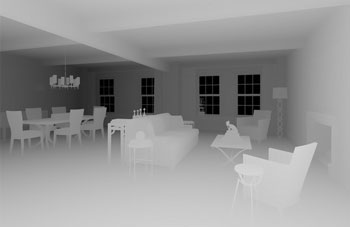
\includegraphics[width=0.6\linewidth]{literature/depth.jpg}
    \captionof{figure}[Example of a depth image]{Example of a depth image \cite{depthimageexample}}
    \label{im:depthexample}
\end{Figure}

Even though there are multiple technologies that can be used in order to calculate these 
distances \cite{lidarinselfdrivingcar, stereovision, DepthFromMonocularImage}, they still have 
the similarity of culminating those distances in the form of a depth map. These can then be 
used in a variety of applications, one of which could be an RL agent. 

Using depth maps as a state-input for RL agents has been performed before \cite{iowamasterthesis, AirSimDroneNavigation, DepthAndStackResearch}. 
However, studies about whether the application of such depth maps in the context of drone control 
allow the agent to generalize better are still lacking. As described earlier, generalizability using 
RGB images can bring with it some problems that depth imaging could potentially solve. Furthermore, 
what the implications are for this state-representation in the specific task of follow-me behavior 
is also relevant. 


        \section{Theory}
In this section, the relevant theoretical background that is 
essential to the domain of Deep Reinforcement Learning will be introduced. 

\subsection{Reinforcement Learning}
RL is a method that is mostly used in dynamic game-like environments 
where an algorithm receives control of some actions and is required to learn a 
certain behavior \cite{RLBook}. Examples of this can be seen where agents apply RL algorithms to 
Atari games and achieve 
relatively high scores on a selection of them \cite{rlsolvingatari}. Being a type 
of machine learning, it employs a means to map situations to actions according to 
the maximization of a pre-determined numerical reward function \cite{RLBook}. The 
main process of learning is to adapt a decision maker, referred to as an agent, 
according to experiences. Here, an action is performed after which a reward is 
given in 
the form of a scalar value by the environment. 
All the externalities 
that determine what state the agent is in, is defined as the environment. This reward is 
then used as a cue  
to alter the mapping from states to actions accordingly. Using this process allows 
the agent to learn from experience on how to act in order to maximize its reward 
signal. The foundation of RL is based on the collaboration between the agent 
and the environment. For each time step, the agent 
finds itself in a certain state. During this state, the agent has a certain set 
of actions that it can choose from. For each of these actions, there 
is an effect on the environment. After performing a chosen action, the agent finds itself 
in a new state, repeating the process of action-selection. This loop is 
illustrated in Figure \ref{AgentEnv}. 

\begin{Figure}
    \centering
    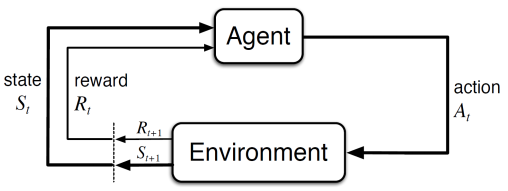
\includegraphics[width=0.8\linewidth]{literature/AgentEnv.png}
    \captionof{figure}[Agent-Environment interaction in RL]{Agent-Environment interaction in RL \cite{RLBook}}
    \label{AgentEnv}
\end{Figure}

The essence of this algorithm is based on the environment's response to each 
action from the agent. During training time, the environment gives 
the agent a reward, possibly in the form of a punishment. The function that 
determines this reward signal, is in turn what the agent will try to optimize and 
therefore, by definition, what the 
agent will try to learn \cite{RLBook}. 

To formalize this process, the agent takes a time-step $t$ which is defined to be a 
single sequence of 
state retrieval, action decision and new state retrieval. This is also written as 
$(S_t, A_t, R_{t+1}, S_{t+1})$.  In this sequence, the agent 
receives a state $S_t$ on which it decides on 
an action $a$ out of the possible available set of actions $A$ using a certain policy $\pi$.
Performing this action changes the environment and provides the agent with a 
new state: $S_{t+1}$. The environment also 
provides the agent with a reward $r_{t}$. By finding an optimal policy $a = \pi(s)$ 
that maximized this reward signal, the agent learns new behavior. An important aspect to consider 
for the agent, is the consideration 
of future rewards as well, which is 
recorded in the return $G_t$ of a certain action in a specific state. 
However, what actions will be chosen by the agent is dependent on the policy $\pi$
that the agent employs. The policy is defined as a probability distribution over
the possible actions for each state. Therefore, by defining an optimal policy 
that maximizes the return, the goal is achieved. 

A crucial concept in RL algorithms is the balance between exploration and exploitation \cite{RLBook}. 
When the policy is completely directed towards exploitation, the agent will 
not explore many of the other possible actions that can be taken that could 
potentially lead to higher returns. Instead, it simply tries to maximize its 
reward signal as much as possible from what it already knows about the world. However, 
there are potentially new states that the agent could explore that could yield 
higher returns. It would therefore be wise to explore the state-space some more. There is a 
strong interplay between exploration and exploitation during the training time of an 
agent that determines how much reward the agent will eventually be able to gather. 
The policies which perform the best are 
the ones that are able to balance both of these strategies in order to maximize 
the overall returns. 

\subsection{Q-Learning}
There are multiple ways in which to implement the learning algorithm in RL \cite{RLBook}. 
One of the more popular approaches, is the method of $Q$-learning. This 
method is characterized by keeping track of the value of performing each action during 
each state. Each action-state pair's value is defined to be the $Q$-value which 
is represented as the expected return for choosing an action $a$ in state $s$, 
expressed as $Q(s, a)=\mathbb{E}_{\pi}\left[R_{t} \mid s_{t}=s, a_{t}=a\right]$.
Intuitively, the expected return is the total sum of expected reward that will be 
collected by choosing this action and continuing from there onwards. This leads to 
the following simplified recursive equation:

\begin{equation}
    Q(s, a)=r+\gamma \max_{a^{\prime}} Q\left(s^{\prime}, a^{\prime}\right)
\end{equation}

The function of this equation in the context of $Q$-learning is, therefore, to update the 
$Q$-values throughout
the learning process where different action-state pairs are being explored. Since the agent, 
when just beginning, is unaware of what the values are for each action, it is imperative 
that it first probes the environment in order to explore the state-action space. The longer 
this process takes, the larger the size of explored state-action space is, and the more accurate 
the agent's predictions about the $Q$-values can be. 

Since $Q$-values represent the overall return of choosing
an action, this will create a mapping from each state to what the value is of each action in 
this state,
taking into account later state-action pairs. Having this information provides the algorithm 
with an overview of good and bad actions to take in each situation. By then employing a policy 
that 
chooses the action with the highest $Q$-value in each state, which is also called a greedy 
policy, 
the agent is able to maximize the reward signal.

\subsection{Deep Q-Learning}
In many RL applications, including the use of RL as a means to control a drone, there is the  
issue of how states and actions are represented. The implementation of Deep Q-Learning \cite{DQNDeepmind}
pose a solution to this problem, which will be discussed below.

In many domains where this algorithm 
is useful, the state or actions can be either continuous or discrete. In most discrete 
state-spaces, keeping a table of each $Q$-value for each state-action pair is a reasonable 
method to keep track of this information. However, in the case of 
a continuous space, keeping a tabular state-representation would vastly inflate the 
computational costs of 
storage, let alone searching time required to sift through this table. This means that 
there is a necessity 
to represent the action space, not categorically, but as a function. 

Additionally, in some applications, the state space is being represented as an image. Using 
images, which can take up a large range of values per pixel, can further complicate how the 
mapping of state to action values happens. However, more importantly, the location of 
the values become important. Image processing requires the processing of the interrelated 
connections between pixels in its 2-dimensional spaces. These problems necessitate 
different requirements to the function approximation tasks compared to a simple one-dimensional 
state input. \newline

\noindent
\textbf{Convolutions and Neural Networks} \newline 
Neural networks have previously been used in order to perform function 
approximations, especially in the context of RL \cite{rlsolvingatari}. Neural networks 
are a biologically inspired network of digital neurons that make predictions and 
adapt accordingly when presented with a ground truth \cite{neuralnets}. The building 
blocks, the neurons 
themselves, have weighted connections to other neurons. These connections 
are the weighted sums of their inputs and a bias term. During initialization of such 
a network, all of these values, also called parameters, are random. The training process 
is defined by the 
modification of these weights and bias terms in order to fit to the data that it is 
being fed. This process happens by the network producing an output prediction, which 
is then checked according to a ground truth. Using the difference between this ground truth and 
the prediction, a cost value is produced and thereby, a cost function. 
An algorithm is then used that calculates the gradient of the parameters that will minimize 
this cost function, which is also referred to as backpropagation. During a training cycle, 
a batch of data is fed forward through a network 
and a gradient towards better weights and biases is calculated and applied. Iterating 
this process, modifies the network to adapt to the data. More importantly, this 
also provides the network with the ability to generalize to new, yet unfamiliar 
data points. There is a strong trade-off regarding the degree to which  a neural 
network has been fitted to training data. The more the network adapts, the better it 
fits the data and can generalize. Nevertheless, it is possible to overdo this, causing 
the network to fit to the data too much, losing its generalization abilities. This 
phenomenon is called overfitting.  

Using neural networks has been an extremely useful tool in many 
domains \cite{riseofneuralnets, NeuralNetworkApplications}. One such domain is 
computer vision, which deals with different vision tasks such as 
visual recognition, image classification, object localization, and object detection 
\cite{CNNapplications2}. Some of these tasks have seen drastic improvements with the 
introduction of a specific type of neural network called a Convolutional Neural 
Network (CNN) \cite{CNNapplications, CNNintroduction, firstcnn}. CNNs rely on the 
principle of convolutions as an operation on the input. This convolution employs a filter 
(also referred to as a kernel) which is a matrix that is applied to the input pixels as a 
sliding window. Performing this operation on the input, creates a new image which 
extracts specific features, dependent on the filter being applied. In the case of 
a CNN, the goal is to learn relevant filters to be applied on the input, in order 
to make correct predictions. The final layers of a CNN mostly consist of fully 
connected layers, which are identical to the normal neural network architecture as 
described earlier. CNN architectures output a probability distribution 
over all the available classes, where the highest probability class is chosen 
as a prediction. 

The application of neural networks as function approximators in RL has been 
a popular choice \cite{rlanoverview}, but especially so in the case of 
$Q$-learning. The determination process of the state-action pairs and their 
corresponding $Q$-values can be performed using the CNN. 
Instead of a class distribution, the CNN now outputs predictions about 
the $Q$-values of each available action, forming this value approximation method.
By employing a certain policy using these values, different behaviors can now 
be either found or performed.   \newline


\noindent
\textbf{Deep Q-Network} \newline
The combination of using both a CNN (or any other type of neural network as a function 
approximator), as a $Q$-learning algorithm is called Deep Q-Learning. An agent 
employing this is called a Deep Q-Network (DQN) \cite{DQNDeepmind} and
works similar to a normal $Q$-learning algorithm. The agent gathers 
experiences in a certain environment, and stores these experiences in a 
replay buffer. During training time, it samples a batch from this 
replay buffer and performs the feed forward through the CNN. Using the  
outputs from the network to compare against what was actually 
observed during the batch of experiences. With this difference, a gradient 
can be calculated which can be backpropagated through the network to become more 
accurate in its $Q$-value predictions. Iterating this process eventually ensures 
that the agent converges at either a local or global minimum. 
Using samples of experiences as training data is done for a more stable training process 
because a possible danger of using only the latest acquired experiences is that the agent 
will forget learned behavior from older experiences degrading its performance.  Furthermore,
changes in parameters also mean changes in behavior, which leads to new experiences 
and consequently, a bias in the data. The fact that the training batches will always 
contain a proportion of considerably older experiences, assures that the agent will always 
be updated with those experiences as well, enabling overall more stable a training 
process.

Once a DQN has been trained, policy selection is straight-forward because a 
greedy policy can be applied to maximize the current knowledge about the reward 
space. However, during training time, to be able to tweak the 
exploration-exploitation process, an $\epsilon$-greedy policy can be applied. 
This policy selects the actions 
with the highest $Q$-value, expect for an $\epsilon$ proportion of times, 
where a random action is chosen. Maintaining an amount of randomness during 
action selection during training time, ensures that at least some degree 
of exploration will be present. Once the training process has been finished, 
this $\epsilon$ can be reduced to naught, prioritizing exploitation. 


        \section{Research Questions} \label{RQs}
In this section, the research focus of this thesis will be discussed, together 
with the sub-problems that will divide the main problem. This thesis will 
investigate the following question. 

\begin{quote}
    \label{mainresearch}
    Main $-$ \textit{To what extent is the use of Reinforcement Learning in the task 
    of Follow-Me behavior applicable and beneficial?}
\end{quote}

\noindent In order to formalize the 
process of answering this question, the next sub-questions are defined.

\subsection{Directionality}
Since the target object is a dynamic moving object, the need to implement some type 
of directionality information, as described in Section \ref{directionality}, in 
the state representation is required. In this thesis, the choice has been made to 
implement a stack of images as means to convey this information.
Doing this could improve the training process, in speed and convergence, and could 
also alter the way in which the follow-me behavior is being performed. From the 
literature, it is still 
unclear whether the agent will be benefited by adding this in the input regarding 
successful follow-me behavior. In order to investigate this, an implementation 
of an agent trained on state-representation containing directionality will be tested 
to answer the following question. 

\begin{quote}
    \label{research1}
    1 $-$ \textit{Does the implementation of stacked images as state-representation improve 
    an RL agent's training and performance in follow-me behavior?}
\end{quote}

\subsection{Obstacle Avoidance}
The desired behavior would preferably not only be to follow a person, but to also 
successfully identify and avoid objects that are in the way. Therefore, we will 
implement a type of state-representation that can convey to the RL agent information 
about where potential obstacles are. For this, state-representations will be changed from 
normal images to depth maps as an implementation of this object sensing. Implementing this, 
allows us to see whether this has 
an influence on the training process or the learned behavior and help answer the second 
research question. 

\begin{quote}
    \label{research2}
    2 $-$ \textit{Does the implementation of dept maps as state-representation improve 
    the performance of the RL agent in the context of follow-me behavior?}
\end{quote}

\subsection{Baseline Comparison}
Another aspect that will be investigated is the benefit of using Reinforcement Learning 
compared to a baseline model. Overall, the goal is to see whether Reinforcement Learning 
works in the context of follow-me behavior. An interesting approach to answering this 
question is to see how the best working RL agent works compared to a pre-programmed 
baseline model similar to the techniques used in previous studies. 

\begin{quote}
    \label{research3}
    3 $-$ \textit{Does the use of Reinforcement Learning provide any benefit over a 
    baseline agent?}
\end{quote}

\subsection{Generalizability}
Finally, to see whether the agent is able to generalize its learned behavior to new,  
more complex environments, the agents will be tested in previously unseen situations.
By training agents in environments where systematic obstacles have been added and 
consequently testing them in more complex environments, conclusions can be drawn 
about how much of the behavior from the previous environment is transferred. 

\begin{quote}
    \label{research4}
    4 $-$ \textit{Do Reinforcement Learning agents generalize their behavior in
    an unseen and more complex environment?}
\end{quote}




        \section{Methods}
This section will be an examination of the experiments that will be performed to answer 
the research questions, as well as the implementation to do so. First, the software that was 
used to build the foundation for the RL framework will be discussed. Next, the implementation 
of the RL framework will be explained. Furthermore, the metrics and the experiments 
will be explained. 

\subsection{Architecture}
Each part of the architecture that will be used for the training and testing of 
the agent will 
be addressed. An overview can be seen in Figure \ref{architectureoverview}. \newline

\begin{Figure}
    \centering
    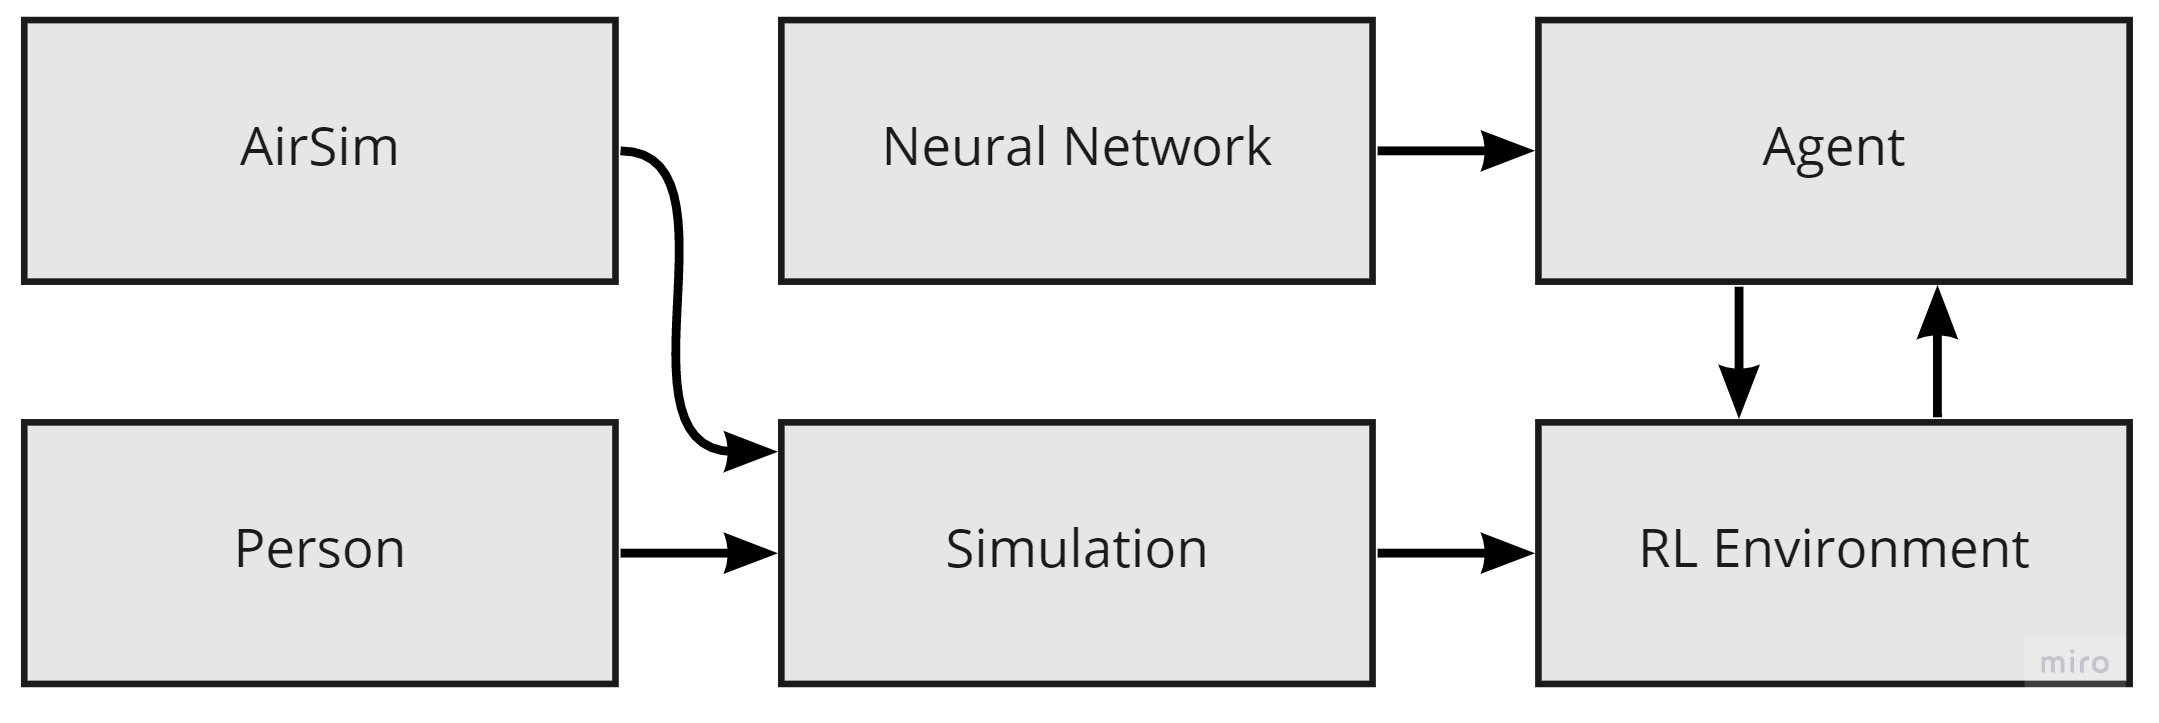
\includegraphics[width=\linewidth]{methods/Pipeline.jpg}
    \captionof{figure}{Overview of each element in the architecture used to perform 
    the experiments in}
    \label{architectureoverview}
\end{Figure}

\subsubsection{Simulation}
The most important aspect of the framework and architecture is the simulation system 
in which the drone will operate. As seen in Figure \ref{architectureoverview}, the 
simulation is the most crucial aspect in which the RL framework operates. The 
simulation is a combination of multiple aspects that will be discussed further, namely 
the person, AirSim and the physics engine defining the physical environment of the drone. 
Each aspect of the simulation environment will be discussed in the coming sections. \newline 

\noindent
\textbf{AirSim} \newline
The program that will be used to take control of a drone will be Microsoft's  
AirSim \cite{airsim}. AirSim is a coding library that is used in order 
communicate with drones instantiated in simulation environments or physical drones. 
Next 
to this, the program allows the user to instantiate a quadcopter directly in a 
virtual environment, together with simulated vision possibilities including a 
normal camera and depth-view. These views can be observed at the bottom of 
Figure \ref{airsim}.Furthermore, using the Unreal Engine \cite{unrealengine}, 
this program allows for a multitude of created environments to be used. This feature 
allows the ability to create or use different environments that systematically introduce 
variables to be tested.  What is more, AirSim has the ability to 
command the vehicles through a Python or C++ script, which makes AirSim very suitable 
to perform Deep Learning. What makes it even more attractive, is that AirSim allows 
easy connectivity with the PixHaw API, which makes it easy 
for the drone to be implemented on an actual physical drone in order to allow 
development for real-life applications. \newline

\begin{Figure}
    \centering
    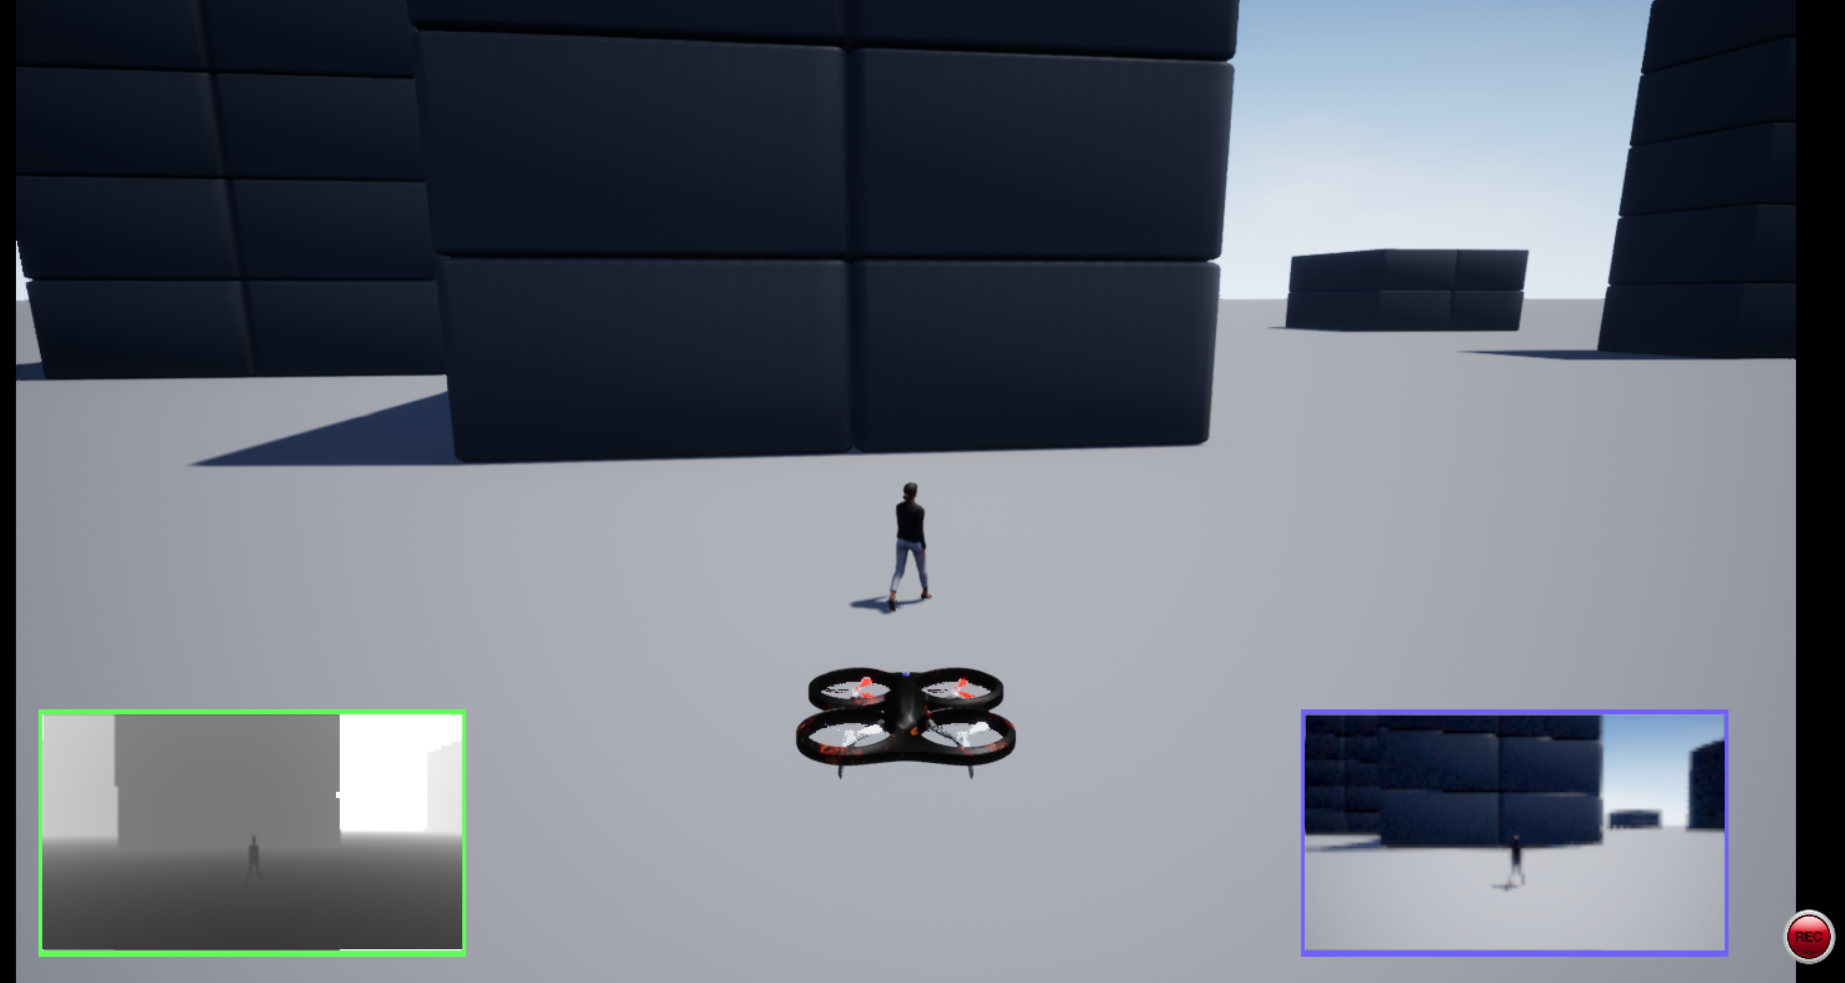
\includegraphics[width=0.8\linewidth]{methods/airsim.png}
    \captionof{figure}{The AirSim program features}
    \label{airsim}
\end{Figure} 


\noindent
\textbf{Environments} \newline
Another aspect of the simulation, is the physical environment in which the drone 
will fly. For this, three environments have been created. A set of agents will 
be trained and tested in each environment which will be specified in Section \ref{experiments}.
Snapshots of the environments from the top view are visible in Figure \ref{routes}.

\begin{Figure}
    \centering
    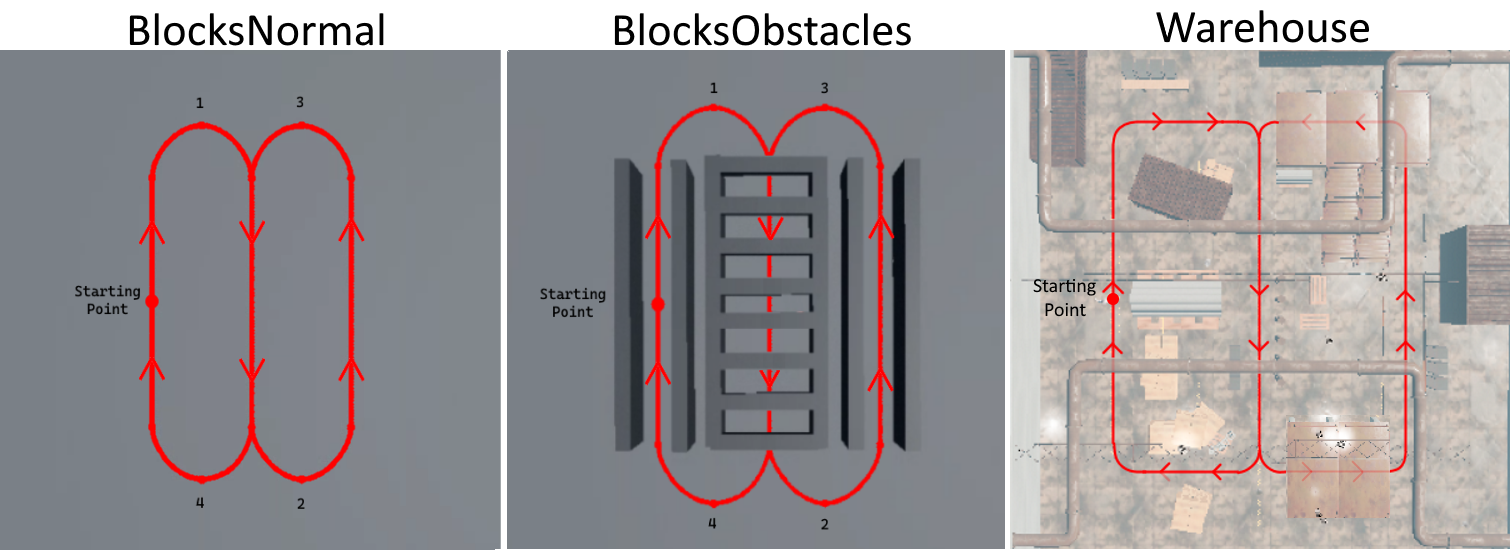
\includegraphics[width=\linewidth]{methods/WalkingRoutes.png}
    \captionof{figure}{The layout and obstacles for each individual environment and the 
    walking path of the person}
    \label{routes}
\end{Figure} 

The shape of the person's walking path inside of the environments are kept a steady 
variable. This shape was picked as a means of balancing the amount of time the person 
will be walking straight and making turns. At the same time, in order to keep an even amount of 
right and left turns, the need to have two left and right turns was kept in mind. For the 
Warehouse environment, a variation 
was used, where the turns of the person were expanded. 
Keeping the walking routes the same eliminates this variable as a possible explanation 
for why certain models might perform less well in certain tests. 

The people that the drone will be following can vary per environment. As will become clear 
in Section \ref{inputs}, the input states will not contain any information about 
the specific individual that is being followed. For this reason, during training time and 
testing time, a different target person can be implemented. Nonetheless, at any point in 
time there will be at most one person in the environment, which will be the person that 
the drone will have to follow. Again, in order to isolate the required task of the 
agent to follow an individual person, the choice has been made to not include multiple 
people. 

Looking at the implemented environments, the first environment will be BlocksNormal, which will 
consist of no obstacles for the 
agent to deal with. In this situation, the agent's ability to learn the follow-me behavior 
will be assessed. The second will be BlocksObstacles in which different types of 
obstacles have been added to simulate three different situations, namely: tight 
hallways, wide hallways and corners. Their locations can be seen in Figure \ref{areas}.
In this environment, the agents ability to deal with these situations will be gauged.
Finally, the Warehouse environments will contain similarly designed situations, 
however with much more details. Here, the objects consist of different types of 
objects and textures but create similar obstacles for the drone to avoid as in the 
BlocksObstacle environment. In this way, the behavior can be analyzed specifically by 
looking at how the agent deals with each specific situation to see whether the agents 
are able to generalize their behavior to new situations.


\begin{SCfigure}
    \centering
    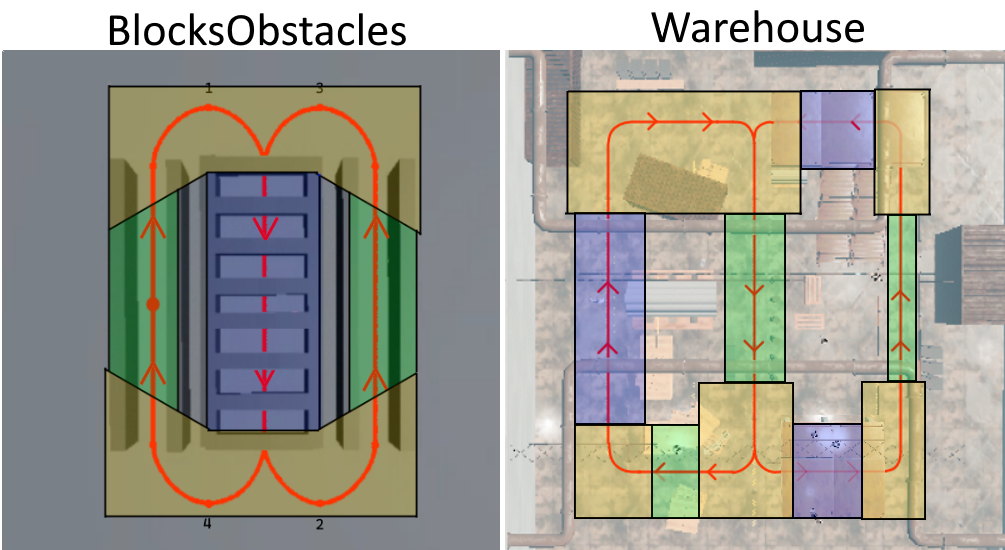
\includegraphics[width=0.66\linewidth]{methods/situations.png}
    \captionof{figure}[Locations of each type of situation in the environments]{Locations of each type of situation in the environments\newline\newline
    The areas correspond to the following situations: \newline
    Green = Tight hallways\newline
    Blue = Wide hallways \newline
    Yellow = Corners\newline\newline}
    \label{areas}
\end{SCfigure}


\subsubsection{Agent Structure}
In this thesis, a DQN will be implemented as an agent that will perform $Q$-learning. 
The choice for this type of learning has been made because 
of the aforementioned reason that the DQN can easily be implemented to be tested in 
new domains. Furthermore, its inputs are easily changed as necessary for the experiments that 
will be run. Now the overall architecture of the agent, which is the decision making body 
that is actually in control of the drone, will be described. \newline

\noindent
\textbf{Inputs} \label{inputs} \newline
The camera inputs of the agents will have a resolution of 128 x 72. Next to this image, the 
bounding box of the person in the view of the drone will be derived. This will provide 
the drone with information about the location and distance of the person in its camera view.
The bounding box will be retrieved using AirSim's Segmentation maps. These maps provide the 
same image as the view from the camera of the vehicle, but instead each pixel represents what object
is in view. An example of one such segmentation maps can be seen in Figure \ref{segmentationmap}. 
The color in this segmentation map for the person is preemptively set during initialization of the 
entire program, and when the drone receives this frame, it searches for the pixels corresponding 
to this color. When this is available, simply taking the extremes 
on both axes will provide the agent with the bounding box of the person. The pixels in 
this bounding box 
area will then all receive a -1 value while the rest of the image will be processed according 
to what type of combination of state-representation is chosen. These images could be 
stacked, which would result in the repetition of this process three times. The image 
itself could also be a depth map, in which case no further processing is done. If the image 
is a normal RGB image, it is first grayscaled. Doing this removes the three channels 
in an RGB image while still maintaining all of the required information. Before passing this 
state to the agent for training and 
decision making, the image is normalized in order to stay within a range of 0 to 1. An important 
note here to make is that the range of the bounding box in the image will stay -1, making the 
possible values for each input to the agent range between -1 and 1. This normalized image is 
then used as an input for the agent to decide on what action to take. \newline

\begin{Figure}
    \centering
    
\includegraphics[width=0.7\linewidth]{methods/segmentation1616512266.6097646.png}
    \captionof{figure}{Segmentation Map from AirSim}
    \label{segmentationmap}
\end{Figure}

\noindent
\textbf{Network and Hyperparameters} \newline
Every type agent will be a variation of the DQN agent and will therefore, contain the same 
network. This network can be seen in Figure \ref{network} and the specific 
architecture details can be found in Table \ref{tab:NetworkArch}. Being quite modest 
in size, this neural network has approximately 2M parameters, 
which makes it computationally easy to train and deploy. 
This architecture has been chosen because of the fact that a convolutional network is required, as 
it is supposed to process image data. However, it does not require to be a large network as the 
limitation of this thesis is that it should stay resource efficient. Furthermore, it is only required 
to make decisions upon these images, so the network architecture does not necessitate a network 
that is extremely large. The optimizer that will be used is Root Mean Square Propagation 
(RMSProp) \cite{rmsprop} with a learning rate of $0.001$. \newline

\begin{table}[h]
    \centering
    \caption{Network Architecture of the DQN}
    \label{tab:NetworkArch}
    \begin{tabular}{l|c}
    \multicolumn{1}{c|}{\textbf{Layer}} & \textbf{Parameters}                                \\ \hline
    Convolutional layer                 & 32 Filters of 8x8 and stride 4                     \\
    Convolutional layer                 & 64 filters of 4x4 and stride 2                     \\
    Convolutional layer                 & \multicolumn{1}{l}{64 filters of 3x3 and stride 1} \\
    Fully connected layer               & 512                                                \\
    Fully connected layer               & 128                                               
    \end{tabular}
\end{table}


\begin{Figure}
    \centering
    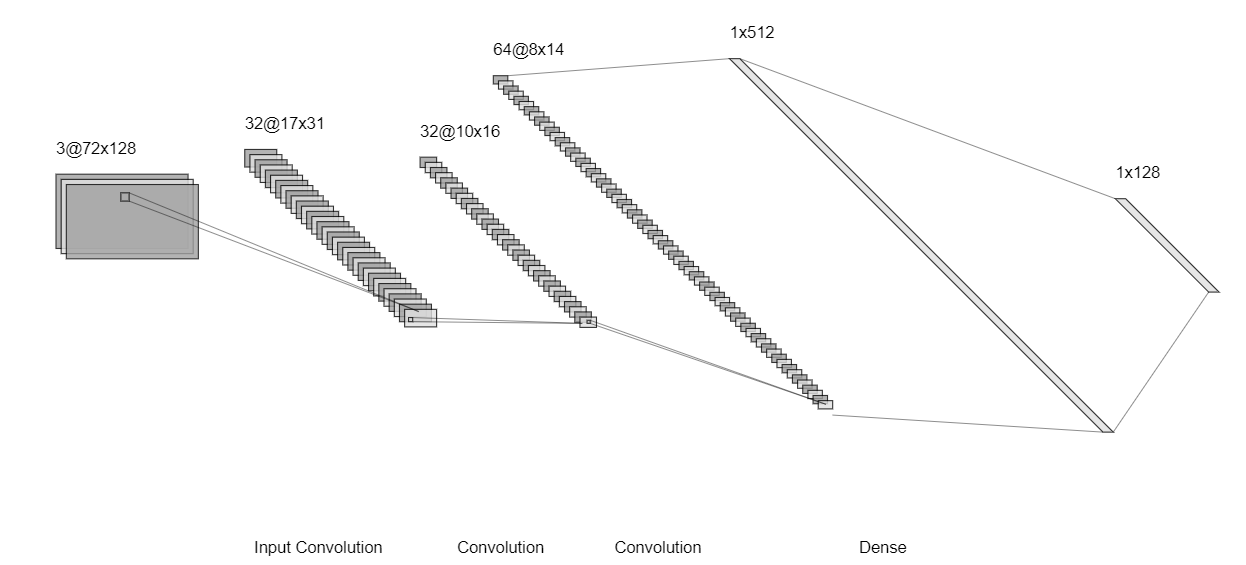
\includegraphics[width=\linewidth]{methods/network.png}
    \captionof{figure}{Network Architecture}
    \label{network}
\end{Figure}

\noindent
\textbf{Outputs} \newline
The DQN's output will be an integer
between the range of 0 and 5, each of these representing an action as is illustrated in 
Table \ref{fig:actions}. These actions have been chosen so that the agent is able to 
manoeuver in the environment in most directions. The ability to orient itself 
is a requirement in order to change its direction. However, this orientation is only 
possible on a horizontal axis. Vertically, the drone will remain at a static height. Its 
vertical orientation is unable to change as these movements would also result in a horizontal 
displacement. Changing the camera positions is synonymous with moving the drone itself. 
An important note to make is that the drone is unable to move backwards. The reason for 
this lack of movement is because the drone is unable to sense what is happening in the 
back. Nonetheless, the movements to the right and left have been included because the drone 
is able to partially observe the obstacles in these settings. 

\begin{table}[h]
    \caption{Mapping from network output to actions}
    \label{fig:actions}
    \centering
    \begin{tabular}{ll}
    \textbf{Integer} & \textbf{Action} \\
    0                & Do nothing      \\
    1                & Orient right    \\
    2                & Orient left     \\
    3                & Go straight     \\
    4                & Move right      \\
    5                & Move left      
    \end{tabular}
\end{table}

\subsubsection{Agents and variations}
In order to answer the research questions (\ref{RQs}), a variation of the DQN will 
be implemented. There will be two types of agents and an additional of two variations that 
will be used in this dissertation. Each of these variations will be introduced and discussed 
here. \newline

\noindent
\textbf{Baseline} \label{baseline} \newline 
First, a baseline that does not use RL techniques but more straight forward heuristics 
to decide on an action will be implemented. The method used for this, has been inspired by the 
techniques that are used in drone control when RL is not used, as discussed in Section 
\ref{baselineliterature}. These methods use the simple assumption that the drone is 
tracking the object when a set of conditions are met. These conditions include that the 
object is centered inside of the camera input and that the size of the object corresponds 
to a certain proportion. From these conditions the distance to the object can be derived 
and whether the drone is looking at it. 

Using these principles, the following agent has been developed. 
With the received camera input, the baseline agent determines where 
the bounding box is in the image. If the center of this bounding box is in the left side view, 
the agent will rotate left. If the bounding box is in the right side of the view, 
the agent will rotate right. If the bounding box center is within a range of the center 
of the view, the agent will check what the height of the bounding box is to see how much it 
differs from the goal height. The goal height being 20\% of the image height, an additional 
margin of error will be permitted in order to prevent constant movements of the agent. In the 
case that the bounding box height is within this margin of 25\%, 
the agent will not move. In the other case, the agent will move forward, coming closer to the 
person. 

Using these methods removes the 
need to perform calculations about the exact location of the person, while also maintaining 
sufficient distance from the person. At the same time, as will be elaborated upon in 
Section \ref{rewardfunction}, these values have been fine-tuned with the reward function in order 
to also maximize the reward function using this method. This agent does not require any training 
and is therefore simply used as a baseline model in order to compare the RL models to. \newline

\noindent
\textbf{State-representation variations} \label{stackedimages} \newline
The RL agent that will be used will be a DQN. However, its state can vary and these will 
be tested accordingly. In this thesis, two such variations will be implemented and investigated.

The first variation to the state-representation that can be made is the use of stacking.
Considering the limitations of this study to maintain a low computationally functioning agent, 
the decision has been made to opt for video input as a means to communicate directionality to the 
agent. The use of RNNs, would require too much computing power. This has been implemented 
by taking three consecutive frames from the environment with 0.1 second intervals
as a means to form a video. This video can also be considered a stacked image of the last three 
frames. This stacked image can be created by getting a frame from 
AirSim (either normal or depth), deriving from it the bounding box, 
processing it as described in Section \ref{inputs} and then finally, simply to stack 
them in a 3-dimensional image as can be seen in Figure \ref{pipeline}. This object is now used 
as the input for the agent.  

\begin{Figure}
    \centering
    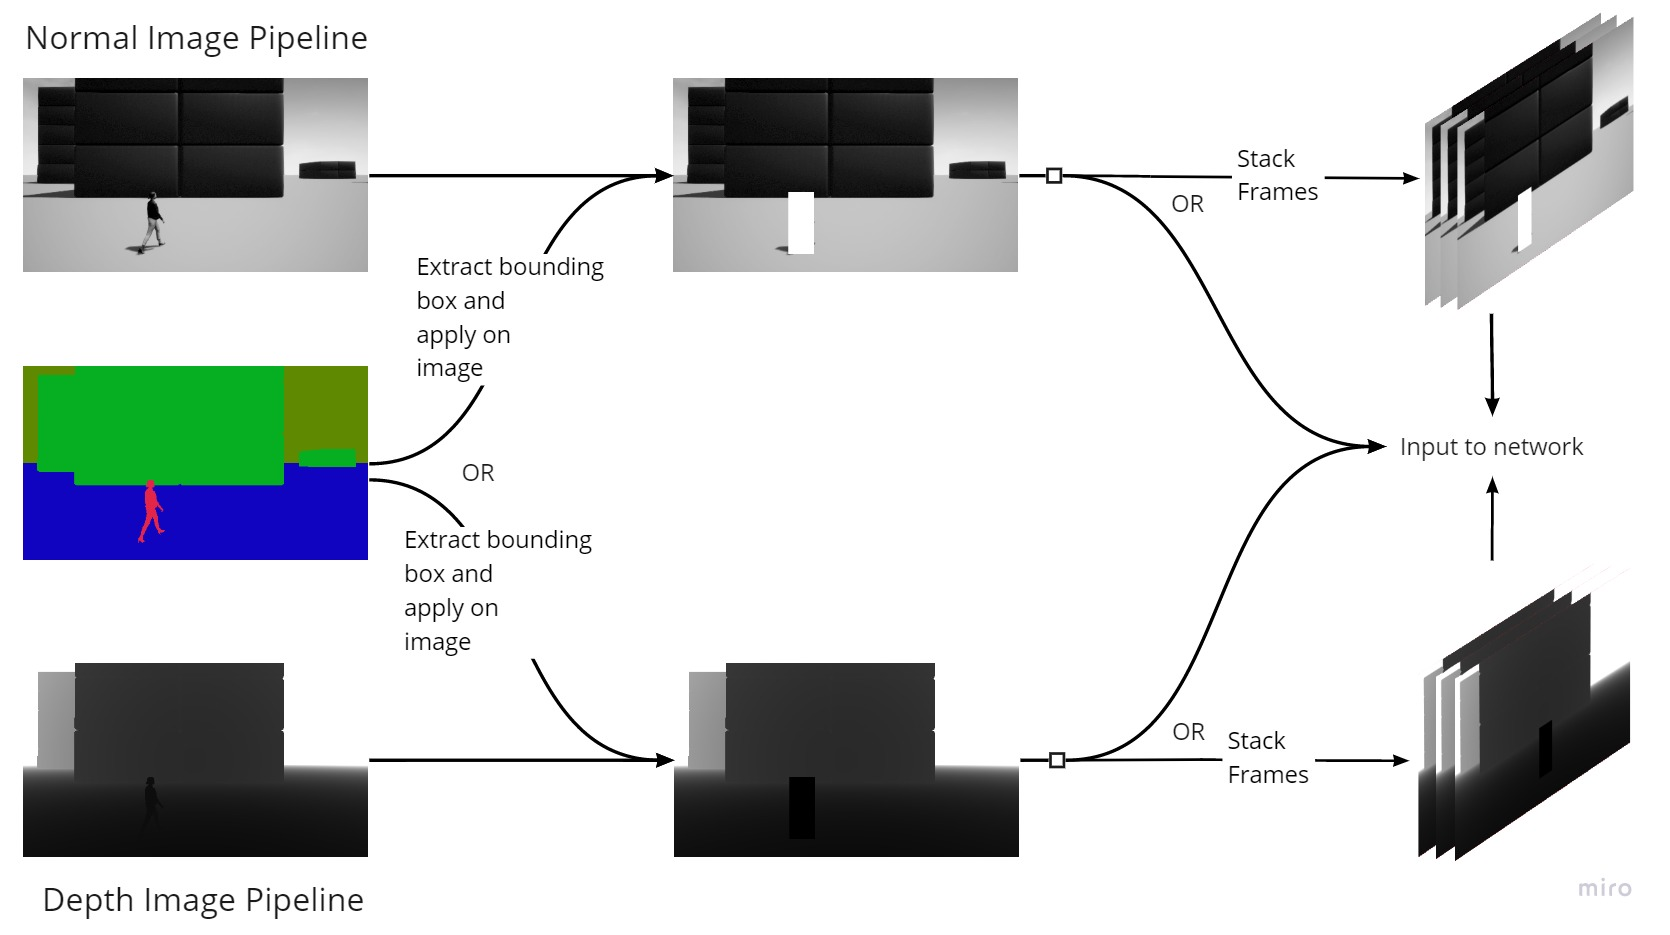
\includegraphics[width=\linewidth]{methods/StateProcessing.jpg}
    \captionof{figure}{Pipeline to process AirSim images in order to create a state for the 
    DQN agent}
    \label{pipeline}
\end{Figure}

Another variation is the use of depth images. 
In order to allow the agent to sense obstacles in its surroundings, the choice has been made 
to us depth maps. This option combines the ability for the agent to receive image input, 
perceive the person and detect the distances to the obstacles around it. AirSim provides 
the ease of simply requesting depth maps from the environment, giving the agent access to 
the ground truth distances to all of its surroundings. Important to note, these depth 
maps can easily be combined with the stacking of them, allowing for all of the possible 
combinations of these agents to be tested.  \newline

\subsubsection{RL Framework} \label{RLframe}
The reinforcement learning framework are also an important part of the implementation that 
require some discussion. The use of a python library that builds 
upon the machine learning library Tensorflow, called TF-Agents has been opted for. Tensorflow is, 
in itself, 
a library that abstracts machine learning algorithms to be implemented. Adding to this,  
TF-Agents allows for a high-level abstraction of the RL implementations. Nonetheless, 
more specific RL environment aspects require to be developed, each of which 
will be elaborated upon in the next sections. \newline

\noindent
\textbf{RL Environment} \newline  
An important aspect of reinforcement learning is the RL environment. Here we refer not to 
the simulated environment where the drone is flying in, but the RL environment that creates 
the states 
and returns rewards where necessary, as seen in Figure \ref{architectureoverview}. The agent 
interacts with the RL environment, which again interacts
with the simulated environment in order to get the required information. Crucially, RL algorithms 
tend to operate in episodes. An episode is characterized by a beginning state and a terminal state, with 
transitions of steps that the agent is taking in between. After this terminal state, the environment 
resets and a new episode begins. 

In this implementation, the starting state of the person is directly behind the person at a 
slight distance. Keeping this initial distance from the person removes a bias in reward in 
earlier states of an episode. After this, a step is taken by the agent. This step process 
is defined as follows. First, a state is retrieved, which is performed as described in Section \ref{inputs}. 
Consequently, an action is chosen by the agent according to this state after 
which a reward is calculated for this new state. Finally, in each step, an assessment will be made as 
to whether an episode has ended, to determine whether the terminal state has been reached. 
This will be done by checking whether one of the next three requirements have been met: the agent 
has collided with an object, the agent has no bounding box in its camera, meaning the person was 
lost from its view; more than 50 steps have been taken. These conditions ensure that an episode 
consist of a finite sequence of actions for the DQN to be able to learn from. Between these episodes, 
the environment resets. This reset makes sure that the drone is reinstantiated 
to the correct position. In this case, the drone is being positioned directly behind the person and 
made sure to be oriented towards the direction of the person as well. These resets are meant as means 
to not waste time in state-spaces during training time that are not conducive for the agent to learn. 
States where it has collided or loses sight of the person are not relevant for the drone in order to 
learn how to follow successfully. Therefore, before too much time has been lost in these states, the 
environment resets to a moment from where it can continue its learning process successfully. \newline

\noindent
\textbf{Training} \newline  
Before the models can start training, some preparatory steps are performed. DQN requires a replay 
buffer where it stores a large dataset of 
experiences. This is necessary for the DQN as it requires samples from this buffer as an input 
for the network for each training step. Since this would also cause the primary training steps to be 
skewed, it's necessary to fill part of the replay buffer before training begins. Therefore, before training 
is started, an agent that performs random actions moves about in the world for 500 steps, filling 
a portion of the replay buffer, which has a size of 10,000 experiences total. This makes sure that an initial portion of the state-space 
is explored already before training begins.  

Next, the training process can be described as a loop where the same steps are being taken each time, 
also referred to as an epoch. 
This loop starts by performing 50 movements in the environment. These 50 movements correspond to a full 
episode before the environment resets. Some of the earlier episodes might not reach their 50 steps 
limit, however, nevertheless, a total of 50 steps will be taken before the network is trained on 
these experiences. This stabilizes the increase in replay buffer size throughout each epoch. 
The batch size of a sample is 64 and each model will be trained either to convergence or 
2000 epochs. 

It is important to note that the TF-agents library maintains two policies for an agent. One
collect policy which is meant to always keep a degree of randomness in order to always keep some 
level of exploration. Next to this, is an evaluation policy which is the optimal policy the 
agent has learned. Every 50 iterations, an evaluation step is taken. Here, 10 episodes are 
being played by the evaluation policy. The required metrics, as discussed later, are stored and 
the training loop continues. \newline

\noindent
\textbf{Reward Function} \label{rewardfunction} \newline  
The most important aspect of RL is the reward function. Since learning in this context depends on the 
maximization of the reward function, the behavior that the agent will learn is highly dependent 
on this reward function. In this thesis, the choice has been made for an easily-developed sparse reward 
function. This is because, as mentioned before, there is no need to imbue the agent with pre-determined 
knowledge about how to reach the goals. This will allow the agent freedom in interpretation about 
how to solve this problem and not limit it to behavior decided upon by the developers. 

The reward function requires a connection from the state input. If this is missing, 
the agent is unable to actually perceive the impact of its actions on its states. To 
solve this problem, the bounding box will be used as an object to determine the reward, 
considering as it contains both information about the relative location as well as the distance 
to the person. Here, similar assumptions as the baseline will be made about relative location of 
the person, as well as its distance. The person should simply be in front of the drone, where 
centering the person in the middle of its camera view is included in the reward function. 
With regards to the distance to the person, a goal bounding box height has been determined 
using the distance to the drone. The goal distance to the person has been determined to be 
four meters, which, combined with the height of the drone, results in the person 
taking up 30\% of the image height. Combining both the centering and the distance 
conditions in a reward function results in the following set of rules. 
 
If there is a 
bounding box and no collision is happening, there are three conditions that are required to be met.
The first of these is the location of the $x$ value of the bounding box center. When this value 
is within a 20\% range of the center of the image, this condition is met. The second condition to be 
met is that the height of the bounding box is within a 30\% range of the goal height.
The final condition to be met is that the location of the 
$y$ value of the bounding box center should fall in the top 80\% portion of the image. This ensure 
that the drone is not positioned too close to the person. 
When all of these conditions are met, the reward is determined to be 1. In case of detected collision 
or a bounding box is missing, a -1 is returned. All other cases return a 0. 

In all of the tests, the reward function is kept a constant, in order to use this 
function as a metric for the performance of each agent. This way, all of the 
tests can be compared measured according to the reward received. \newline

\noindent
\textbf{Metrics and Methods of Analysis} \label{metrics} \newline  
The metrics to evaluate the training process, the follow-me performance and the behavior will be discussed.
Multiple perspectives will be taken. First, the training process is evaluated according 
to certain metrics. Next, overall performance metrics will be used as well. Finally, in order 
to compare the behavior of each agent, some formalizations will be introduced. 

An overall crucial metric, which will be used throughout this thesis, is the average 
return. In this metric the average reward that was gathered in an episode is recorded. 
This metric will be used to evaluate both the training procedure but also the agent's overall 
performance. As this metric encapsulates all of the requirements of the agents behavior, namely 
obstacle avoidance, person centering and keeping its distance. 

Metrics specific to the training procedures are the following. First, next to the average return, 
the average length of an episode
will be tracked. Since the 
episode can end early when a crash happens, or the person is out of sight, the longer an episode 
takes, the better the drone is at following the person. The cap here is at 50 steps, 
since that is when an episodes resets regardless. During the evaluation step there is a variation 
to these metrics. Instead of the average episode 
length and the loss, the minimum and maximum return are being recorded. These express the worst 
episode and the best episode that the model performed. The preferred situation is where the range 
between these two value is not too large. However, if that is not the case, looking at these 
extremes can shed a light on where the model is still lacking. 

With regards to quantifying the agent's behavior, a number of analysis techniques have been used 
to get in-depth information. First, for each of the 50 possible 
time-steps that an episode can last, the average received reward will be recorded. This 
information gives insight into how an average episode progresses for the agents and 
express potential bottlenecks of the agent as it showcases what the distribution is of the 
received reward through an average episode. Next to this, the paths the drone has taken 
throughout the test run and the location and type of episode ending will also be recording. 
This information provides data about the behavior of the agent and in which situations 
it is struggling the most. All of these aspects will be used to draw conclusions 
about the performance and behavior of each individual agent. 


\subsection{Experiments} \label{experiments}
In order to answer the research questions from this thesis a set of experiments will be run 
in the effort to answer them. The experiments will be performed per environment, each of them 
increasing in complexity. First, tests will be run in BlocksNormal, after which BlocksObstacles 
will be used to run tests in. Finally, tests will be run in the Warehouse. These tests together with 
the research question they answer, are illustrated 
in Figure \ref{im:experiments}. Each will be discussed in the following sections. 

\subsubsection{BlocksNormal}
First, four agents will be trained and tested in the BlocksNormal environment. The procedure 
in which this will happen, will interchange training with test sessions. Primarily, a DQN 
with single normal images and a DQN with stacked normal images will be trained. After this, 
both of them will be tested. The best working state-representation will be used for the final 
agent to be trained using depth images. This means that either a single depth or a stacked 
depth image DQN will be trained and tested. Finally, a baseline will also be tested and used 
for a comparison. After all of these tests have been run, the behaviors will be analyzed together 
with their overall performance. This means that each of the agents will be compared to the baseline 
in order to quantify how much better the RL agents perform compared to the baseline. 

\subsubsection{BlocksObstacles}
The second procedure will be performed in the BlocksObstacles environment and this 
will be performed in the exact same order as the previous environment. However, in the end, 
the performance will not simply be compared to the baseline. After the two tests in the 
BlocksNormal and the BlocksObstacle environments, the expectation is that there is a 
degradation in performance. This proportion of degradation will be used to compare the 
decrease in performance of each RL agent as well. Performing this comparison will give insight 
in whether the agents are comparatively better at handling this environment than the baseline. 
Finally, the best working agent in this environment will be retrained using a slightly modified 
reward function. This reward function will have tighter margins. Where the normal reward function 
had a margin of 25 \%, this one will be performed using 10 \%. Performing this test will 
reveal how the behavior can be targeted using the reward function. 

\subsubsection{Warehouse}
Finally, training and tests will be performed in the Warehouse environment. Starting by 
testing and comparing both the best working RL agent from the BlocksNormal and BlocksObstacles 
environment. The better working model of these will be retrained inside of the Warehouse environment. 
Performing these tests will give insights in to how much each agent was able to transfer knowledge from 
its trained environment to this new environments. Comparing these models to the baseline degradation, 
similarly to the previous environments, will again show how much better the RL agents are. 

\begin{Figure}
    \centering
    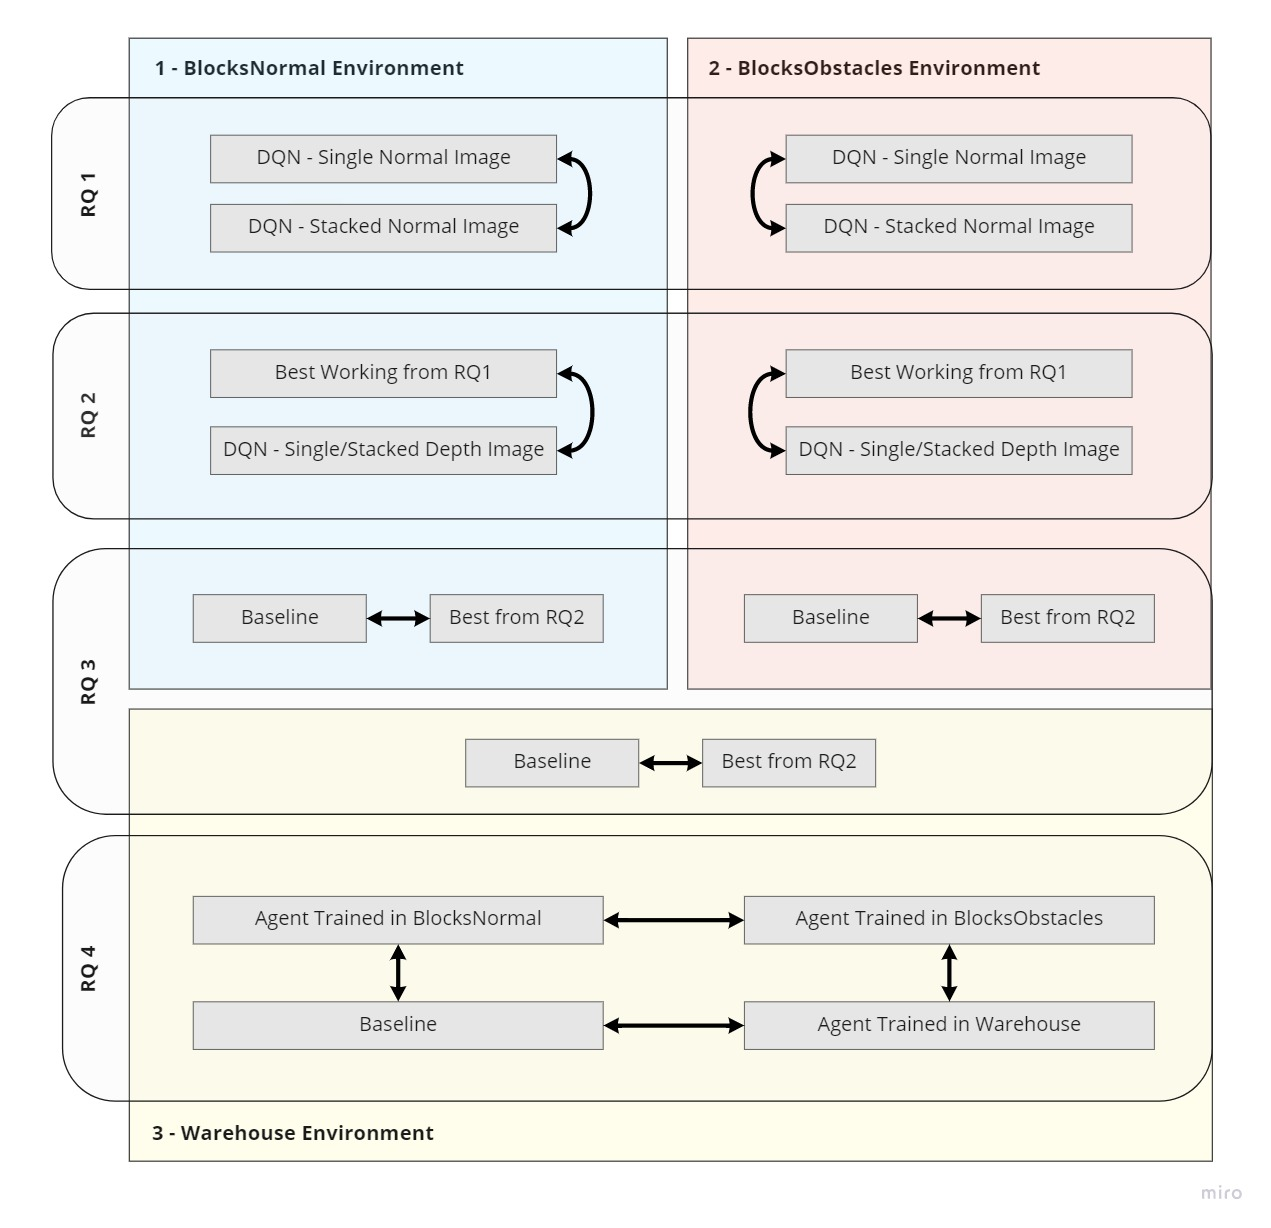
\includegraphics[width=\linewidth]{methods/experiments.jpg}
    \captionof{figure}{Experimental procedure that will be followed. The order will be to start 
    with the BlocksNormal environment, moving to the BlocksObstacles and ending with the Warehouse}
    \label{im:experiments}
\end{Figure}


        \section{Results}
This section will present and analyze the results from the described experiments 
and will be addressed similarly to that structure. However, first, the baseline 
will be tested in each environment in order to establish the complexity of the 
environments beforehand. 

\subsection{Hardware}
The experiments have been performed on a NVIDIA Geforce GTX 980M graphics card, 
with 8GB of RAM and an Intel Core i7-4720HQ CPU with 2.60GHz. The simulation uses a mix 
of both the GPU and the CPU in order to perform the basic operations. The RL framework 
relied solely on the CPU in order to allow the rest of the GPU space to be used for the 
training of the agent. 

\subsection{Baseline Performance}
The initial tests will first be performed by a baseline 
agent. This agent has been run in each environment, in order to see how it performs and 
behaves. The same metrics as for the RL agents will be recorded, and these values 
will be used as a measuring tool for the RL agents. More specifically, the 
degradation in performance with the previous environment will be calculated. After 
having run the tests, these results can be seen in Figure \ref{tab:BaselinesAVG}.

\begin{table}[h]
    \centering
    \caption{Average return of the baseline agent in each environment and the corresponding 
    degradation of performance compared to the previous environment}
    \label{tab:BaselinesAVG}
    \begin{tabular}{l|c|c}
    \multicolumn{1}{c|}{\textbf{Environment}} & \textbf{Average Return (/50)} & \textbf{Difference*} \\ \hline
    BlocksNormal    & 40.2 & -        \\
    BlocksObstacles & 22.9  & -43.0 \% \\
    Factory   & 9.9  & -56.8 \%
    \end{tabular}
    \justify
    \small
    *The difference has been calculated by comparing the average return of an agent with 
    the average return in the previous environment. 
\end{table}

What can be deduced from these initial results, is that the baseline agent 
has more trouble the more obstacles are being added to the environment. With 
the addition of walls in the BlocksObstacles environment, the agent already 
performs considerably worse. However, what becomes clear, is that the
implementation of the agent in an even more complex environment, results in 
an even bigger performance drop. These findings more strongly emphasize 
the weaknesses of baseline implementations: namely their inability to 
deal with obstacles and complex environments. 

In order to further 
investigate how an average episodes is performed by the baseline, a 
reward distribution has been created, as seen in Figure \ref{im:BaselinesDistros}. 
Here the proportion of time that a positive reward signal was received at a 
given step in the episode has been plotted, with the green line representing 
a running average of the last 5 steps. 

\begin{Figure}
    \centering
    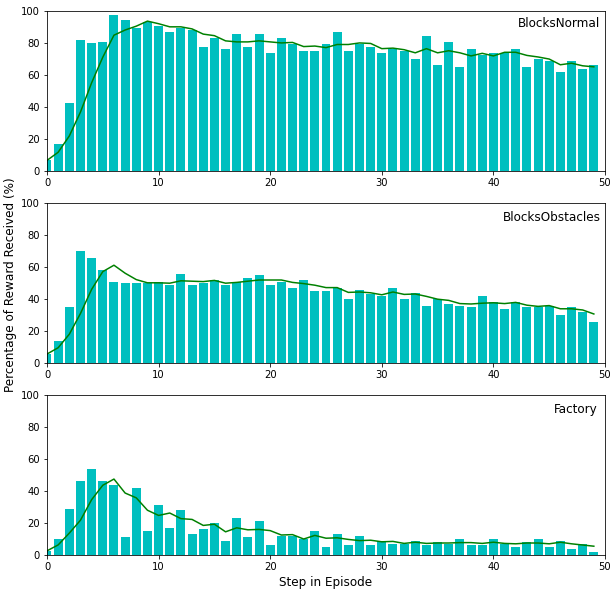
\includegraphics[width=0.8\linewidth]{results/Reward Distribution of Baselines.png}
    \captionof{figure}{Baseline reward distributions in each environment}
    \label{im:BaselinesDistros}
\end{Figure}

The first five frames of an average episode look the same for each agent. This is 
reflected in the image by the sharp increase in reward early in the episode. 
During the first frames, it is hard for the agent to receive  
reward because of the reset distance between the drone and the person. 
Reflected in the figure, the beginning frames contain low values. This 
lack of reward in the initial steps is also the explanation for why the agent 
will never be able to receive an average reward of 50, as receiving a reward 
in these initial steps is extremely hard. The consequent steps,
however, increase drastically, seeing as the drone is approaching the person. 
This behavior happens in each episode because in the first moments, the chances 
that the person will have walked behind an obstacle are slim, resulting in these moments 
where the agent is able to follow. Nonetheless,
it is still very hard to maintain a 100\% reward in each consequent step, as the agent 
sometimes acts slightly too late, resulting in some steps where no reward is received. 
This same pattern is visible in two obstacle environment, however with a proportional 
degradation in rewards in the later stages. This points at the inability of this 
agent to avoid obstacles after the initial run-up to the person. 

\begin{Figure}
    \centering
    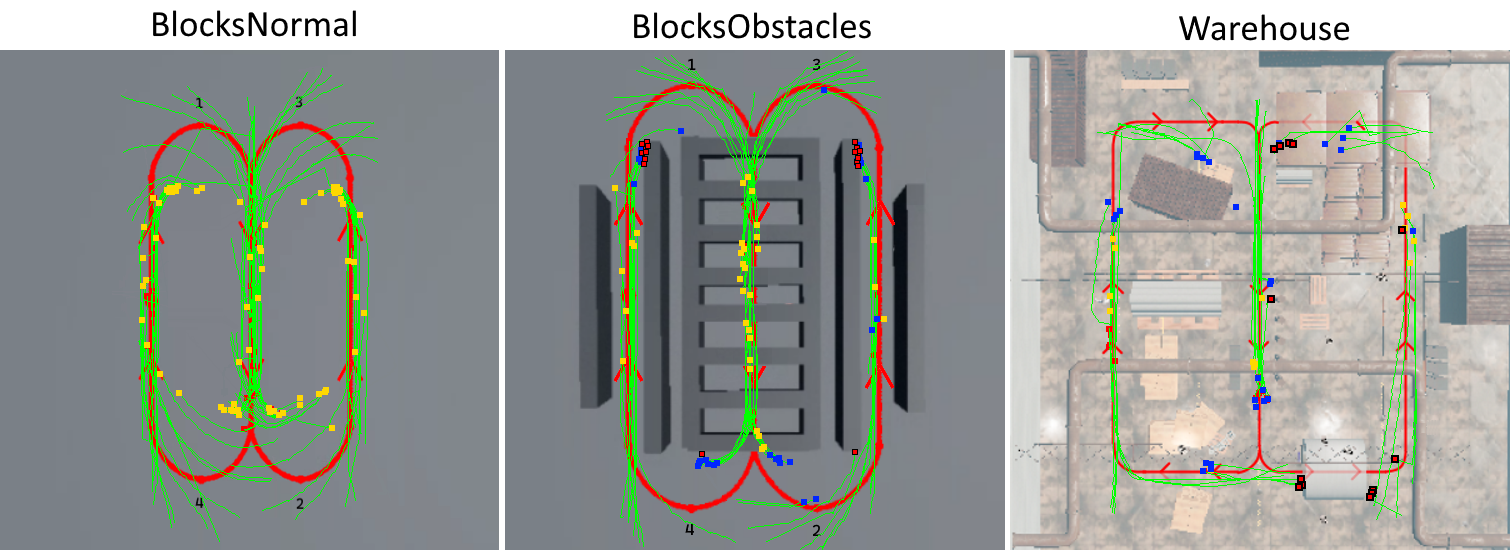
\includegraphics[width=\linewidth]{results/BaselineEnvironmentsPaths.png}
    \tiny 
    Yellow = Normal end $|$ Blue = Out of View $|$ Red = Collision
    \captionof{figure}{Paths and episode ends of the baseline ends during 100 episode test runs 
    for each environment}
    \label{im:BaselinePaths}
\end{Figure}

Looking at the path of the baseline inside of the BlocksNormal environment in 
Figure \ref{im:BaselinePaths}, 
it is clear that the agent follows the paths of the person neatly. During 
the turns, the paths of the agent finds itself inside of the diameter of the 
turn, which is to be expected since in these moments all the agent 
needs to do is simply turn to keep the person in its FoV with the sporadic 
move forward in order to keep the person at the right distance. However, performing 
this behavior inside of the other two environments posed problems for
this agent as can be seen by the increase of collisions and moments of losing 
the person further illustrated by Table \ref{tab:BaselinesEnds}

\begin{table}[h]
    \centering
    \caption{Unsuccessful episode endings of the baseline in each environment during the test run}
    \label{tab:BaselinesEnds}
    \begin{tabular}{l|c|c|c}
    \multicolumn{1}{c|}{\textbf{Episode End Type}} & \textbf{BlocksNormal} & \textbf{BlocksObstacles} & \textbf{Warehouse} \\ \hline
    Out of View           & 0          & 33          & 16          \\
    Collisions            & 0          & 20          & 60          \\ \hline
    \textbf{Total (/100)} & \textbf{0} & \textbf{68} & \textbf{76}
    \end{tabular}
\end{table}

Looking at both 
types of hallways that the agent finds itself, it does not seem to struggle with 
these situations. Both the tight hallways on the outer sides of the walking route
and the wider hallway in the middle of the map, seem to be easy situations for 
the baseline to handle. This makes sense, as the baseline is programmed to simply 
move forward in these situations. It is the corners situation 
where this agent is unable perform adequately. There 
are four clusters where these problems seem to arise. Two at the bottom at the 
beginning of the turn, where the agent keeps losing sight of the person, and two at 
the top where the drone keeps crashing into the wall as well as lose sight of the 
person. Why the agent struggles in these situations is an expression of the fact 
that in these turns, it is necessary to be able to avoid an obstacle. Such behavior 
is not programmed, resulting in failing situations. An example of a failing moment 
can be seen in Figure \ref{im:BaselineLostSight}.\newline

\begin{Figure}
    \centering
    \small
    Image: view of the drone $|$ Arrows: Action the agent performed
    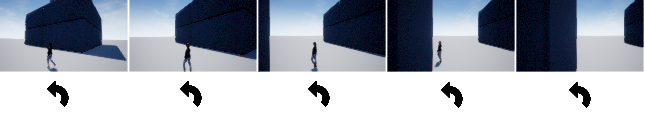
\includegraphics[width=\linewidth]{results/specific_situations/baseline_outofview.png}
    \captionof{figure}{How the baseline loses sight of the person in BlocksObstacle}
    \label{im:BaselineLostSight}
\end{Figure}

Since the person is within the correct distance, the agent does not come closer but 
instead keeps centering the person in its view. However, as can be seen in the last 
three frames, the wall is becoming visible. This does not influence its 
behavior, leading to the person walking behind the wall which makes the drone 
lose sight of the person. The reason why the collisions occur in the 
top two clusters, has to do with the type of situation the drone is in. In the top two 
turns, the drone is leaving tight hallways, where there is less room for mistakes leading 
to early collisions. This is less of a problem in the bottom two turns, where the drone is 
in a wider hallway with more space. 

Finally, looking at the performance of the baseline in the warehouse environments, 
it is clear that the agent has even more problems. As seen in Table \ref{tab:BaselinesEnds}, 
a vast majority of the episodes have ended in either a collision or the drone 
losing sight 
of the person. Looking at Figure \ref{im:BaselinePaths}, it becomes clear 
that the agent struggles in exactly the same situations as in the BlocksObstacles 
environment. The clusters of out of views and collisions happen exactly 
in the same situations as in the BlocksObstacles environment. The exact 
locations can be observed in Figures \ref{im:ObstaclePathsDivided} and \ref{im:FactoryPathsDivided} 
in Appendix \ref{appendixA}.

With these experiments, it becomes clear that the baseline is an agent that works
the best in the BlocksNormal environment, where no obstacles are present. However, 
with the introduction of obstacles, this heuristic method becomes increasingly 
problematic and unable to deal with these new additions to the environment. These shortcomings 
show that the use of heuristic based methods are unable to deal with changing factors, 
unless explicitly programmed to do so.  There is still a benefit for agents to be able 
to adaptively behave according to the environment, which would be the case for RL agents. 
Using this behavior as a control condition in the next experiments enables the drawing of 
concrete conclusions about the specific way in which RL agents are able to outperform 
such a baseline. 


\subsection{BlocksNormal Environment}
In this section, the training and test results of the agents inside of the 
BlocksNormal environment will be discussed. 
First, the training procedure will be addressed after which the test runs 
will be elaborated upon. 

\subsubsection{Training Process}
Inside of the BlocksNormal, a set of agents have been trained. Which variation on the 
agents has been trained has been selected by looking at each consecutive test result. 
After training the single normal image DQN and the stacked normal image DQN, test 
runs are performed to see which performs better. The agent with the higher 
average return is used for the next training session, where it is retrained using 
depth images instead.

The training progression can be observed in Figure \ref{im:NormalTraining}. The data 
of this process has been smoothed in order to observe the underlying trend in the volatile data. 
Meanwhile, the range of the data has also been added in order to still perceive the 
volatility of the training process. 

As has been discussed previously, the training processes is interrupted by evaluation 
moments at each 50 iterations. The differences between training and 
evaluation can 
be seen in the figure. The two main metrics that are 
recorded during training time are the average episode length and the average return 
during each episode, while the evaluation cycles are being observed through 
average return, maximum return and minimum return. 

Initially, the starting points of each average episode length during training are all divergent. 
This happens because the initial parameters of each model are 
instantiated randomly. When this happens, the agent also acts randomly making the probability 
that the drone loses sight of the person low. Losing the person from its view happens because 
the required behavior to lose the person consists of a sequence of the 
same movements, specifically a rotation in any direction. The chances that such a sequence 
occurs under a random acting agent is very slim. As the agents start to learn, new behaviors 
appear, including faulty ones such as sequences that lose sight of the person. This process
is what can be seen in the initial dip that is visible in Figure \ref{im:NormalTraining}.

\begin{Figure}
    \centering
    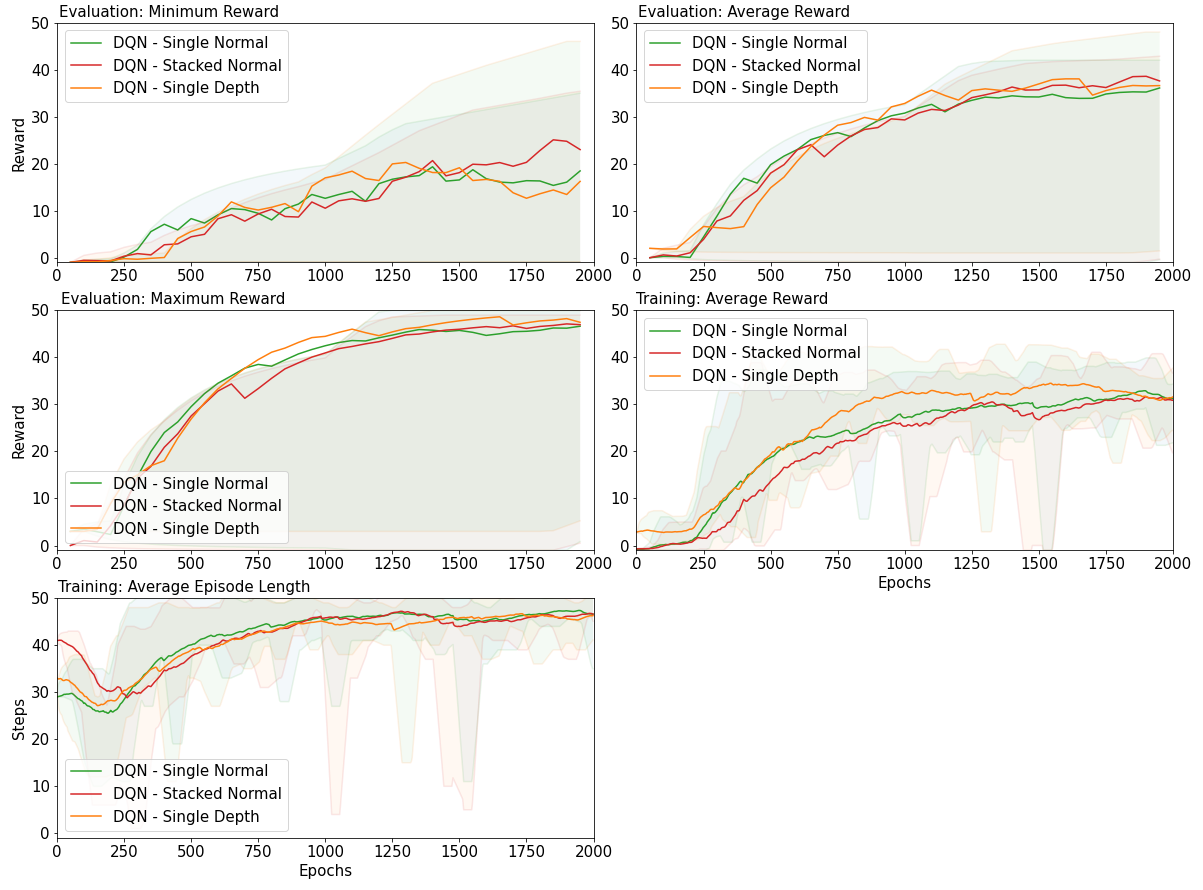
\includegraphics[width=\linewidth]{results/Training for BlocksNormal.png}
    \captionof{figure}{Training Process in BlocksNormal Environment}
    \label{im:NormalTraining}
\end{Figure}

\noindent 
After this, the agent learns better behavior leading to the recovery in the average return.
This dip is not reflected in the average return, because this learning process happens 
before the agent has found the right distances to the person to receive a reward.

Furthermore, during the training process, all the agents were capable 
of converging their average episode length close to the maximum number. Since an episode can 
at most be 50 steps, if the agent is capable of keeping the person in its FoV throughout 
this entire time, the episode length will be 50. Seeing as all the agents are 
able to converge close to this limit, this signifies that the agents have all been able to 
learn how to keep the person in 
their FoV, whatever its distance.
This is reflected 
in the training average return as well, where the curve is similar in shape 
to the average episode length. The longer the episodes, the higher the average rewards that the 
agent is receiving throughout each episode. Being able to 
keep the person in its FoV signifies a first step to learning how to perform the follow-me 
behavior. 

The volatility in the data is explained by the random initialization of the agents. As 
the epochs progress, this volatility reduces, furthermore emphasizing that the agents are 
becoming more stable. 

When it comes to the average return during training cycles, all the agents are able to 
converge to similar values, being around 30. This means that 
out of the 50 steps that the agent is taking, an average of 30 frames were spent in 
goal states. The remaining frames have therefore been spent in states where the person 
was either not centered or not close enough. Comparing this to the evaluation average return, 
this metric converges higher, around 35. The reason 
why this is larger than the training value can be explained with the fact that the 
training cycles happen with a collect policy which includes a certain degree of randomness.
The evaluation cycles are performed using a greedy policy. This means that 
there will always be a slight discrepancy between these two converged values in favor 
of the evaluation average return.  

Looking at the progression of how the agent learned its behavior, 
the maximum value that the agent earned in the evaluation run also converged around 50. 
Therefore, the best episode 
that the agent is able to perform, is one where in most of the steps the agent was 
in a goal state. Considering this, it is interesting to see that the single depth image 
model was able to achieve these near perfect episodes the fastest, compared to the other 
models. The ability to sense the distances between itself and other objects seemed 
to have a positive influence on the training process for the agent in an environment 
where no obstacles are present. 

Finally, the minimum return in an evaluation run is very volatile. This most likely has 
to do with the fact that 
some episodes seem to still confuse the agent enough for it to end the episode very 
quickly by losing it out of sight. Nonetheless, the overall trend of the minimum rewards 
seems to have a positive slope. The final values that all of these agents converge on is 
around 20, which means that the agents have all learned to have a type of behavior that 
at the very least, is able to gather around 20 reward points per episode. 

\subsubsection{Test Results} \label{test_results}
The average return and baseline comparisons of the test runs performed in the BlocksNormal environment can 
be observed in Table \ref{tab:NormalAvgReturn}. 

\begin{table}[H]
    \centering
    \caption{Average return of the agents and performance comparison with the baseline in 
    the BlocksNormal environments}
    \label{tab:NormalAvgReturn}
    \begin{tabular}{l|c|c}
    \textbf{Agent} & \textbf{\begin{tabular}[c]{@{}c@{}}Average return \\ (max. 50)\end{tabular}} & \textbf{\begin{tabular}[c]{@{}c@{}}Compared\\to baseline\end{tabular}} \\ \hline
    Baseline             & 40.2  & -                                                                \\ \hline
    DQN - Single Normal  & 35.2  & -12.43 \%                                                                \\
    DQN - Stacked Normal & 31.9  & -20.64 \%                                                                \\
    DQN - Single Depth   & 42.0  &  +4.5 \%                                                              
    \end{tabular}
\end{table}

Overall, these results show that only some of the RL agents in this environment are able 
to match the performance of the baseline. A surprising result, is that the stacking 
of images did not seem to improve the performance, and had the largest performance 
drop compared to the baseline. This is interesting, as this means that 
although the RL algorithms were able to match the performance of the baseline throughout 
their learning process, the stacked image RL agent did not. Although RL 
is able to teach itself behavior that would be similar to a very straight-forward 
baseline method, the addition of a stacked image state-representation impeded the 
agent so much as to reduce its average return.

Furthermore, the use of depth images instead of normal images did appear to boost the 
agent's performance, enough for an average of 7 frames per episodes and an increase in 
performance compared to the baseline. In order to better understand the behaviors
of each of the RL agents during these test runs, the next sections will focus 
on each specific aspect of their behavior.  \newline

\noindent
\textbf{Reward Distribution} \newline
In order to analyze how each agent performs an average episode and where each agent's 
strongest aspects are, Figure \ref{im:NormalDistro} has been made, 
where the green line represents a running average of the last 5 values.

\begin{Figure}
    \centering
    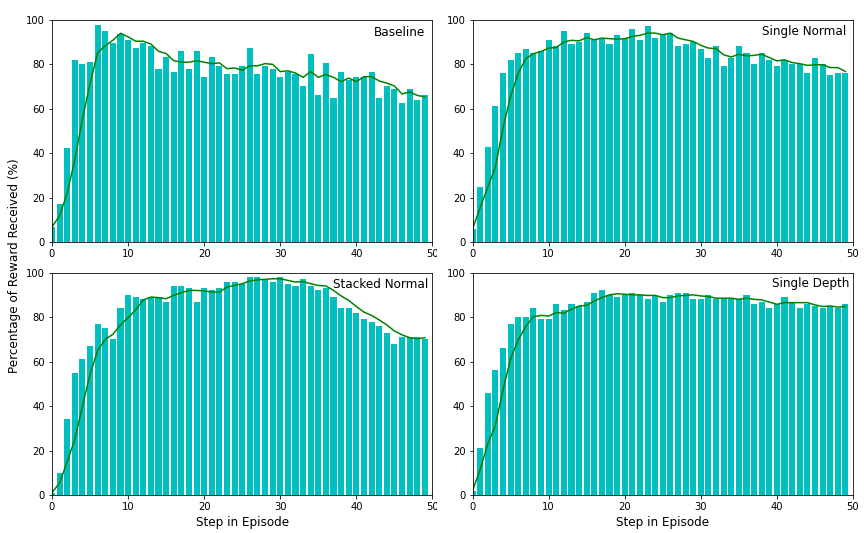
\includegraphics[width=\linewidth]{results/Reward Distribution of BlocksNormal.png}
    \captionof{figure}{Reward Distribution of each agent in BlocksNormal environment}
    \label{im:NormalDistro}
\end{Figure}

As can be seen, there are differences in how each agent performs an average episode. 
Most notable is that, with the exception of the depth agent, most agents struggled with 
keeping a stable reward for longer than 25 steps. Initially, this is not different from the 
baseline and points to the fact that the longer an episode takes, the higher the chance 
the episode ends unsuccessfully. However, the contrast with the depth image is surprising, 
who performs very stable. This shows that the model has learned to 
keep making decisions that allow the agent to stay in goal states on a stable basis.

These results show some 
shortcomings of the RL models which did not use a depth imaging. Both of these agents 
were less stable in their behavior throughout an average episode than the baseline agent. 
In order to analyze what the exact behaviors are that lead to these reward distributions, 
a more in-depth look will be taken at each of them inside of the environment. \newline

\begin{SCfigure}[][h]
    \centering
    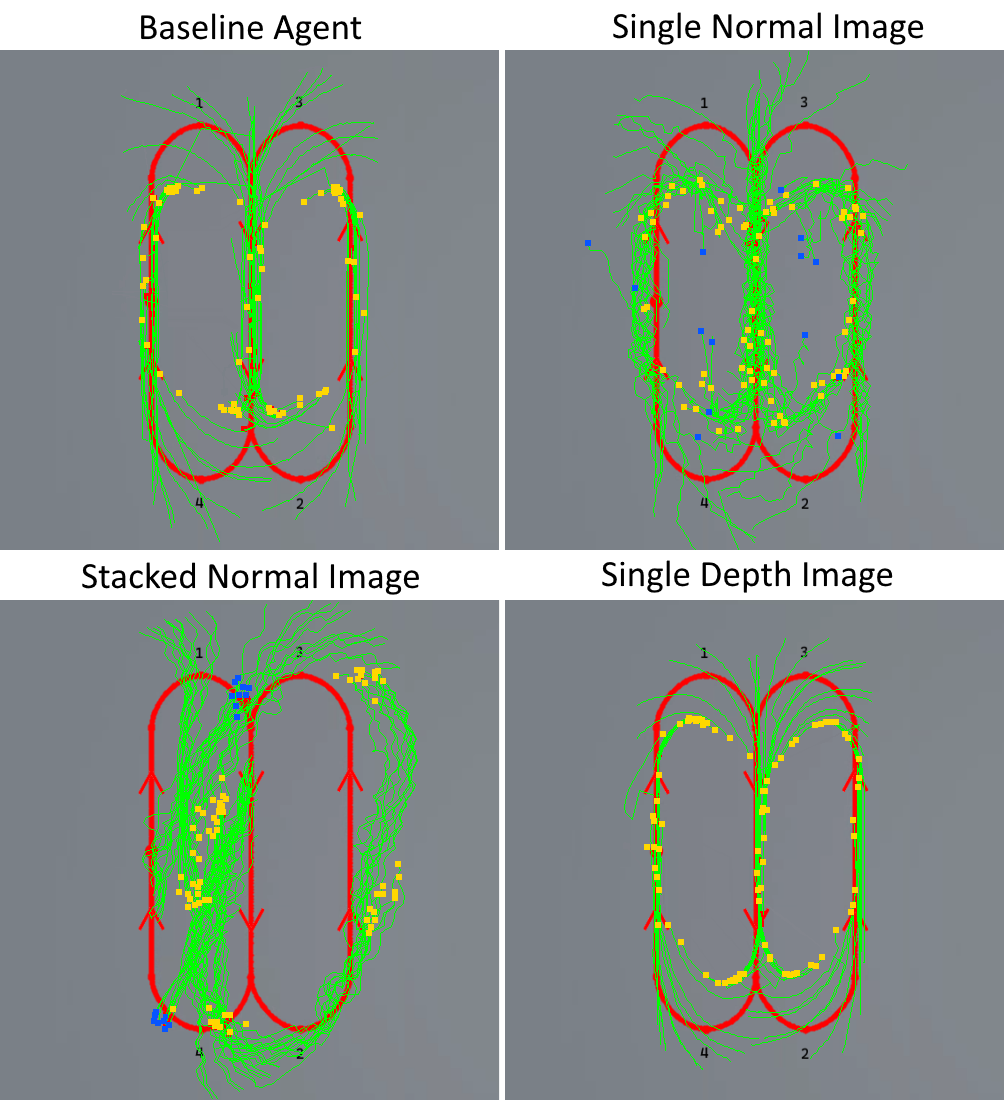
\includegraphics[width=0.66\linewidth]{results/summary-BlocksNormal-Pathsnew.png}
    \captionof{figure}[Paths and episode ends of all the agents during a 100 episode test run in BlocksNormal]{Paths and episode ends of all the agents during a 100 episode test run. 
    The green lines represent the flight paths of the agent.\newline\newline
    The dots correspond to the following episode ends: \newline
    Red = Collisions\newline
    Blue = Out of View \newline
    Yellow = Normal\newline\newline\newline\newline\newline\newline\newline\newline\newline\newline\newline\newline\newline}
    \label{im:NormalPaths}
\end{SCfigure}

\noindent
\textbf{Behavior} \newline
To analyze the overall behavior of the agents, the paths throughout the 100 episode 
test runs have been superimposed over the path of the person. This imposition can be 
seen in Figure \ref{im:NormalPaths}. The added green lines are the path of the agent 
during the episode. The red dots have been the episode ends that occurred through a crash. 
Blue dots indicate the drone lost sight of the person and a yellow dot simply means that the 
episode ended after 50 steps. 

The most notable element in this image, is the contrast that 
the single normal and stacked normal image agents have compared to the 
other two agents. Both of the former agents have very rough flying paths compared 
to the other two. The single normal image has taught itself how to follow the person around its 
paths, but has done so with behavior that is still sub-optimal considering its average return and 
includes a high level of variability. Considering the frequencies of unsuccessful episode ends from 
Table \ref{tab:NormalEnds}, this further emphasizes the weaknesses of this agent. 

\begin{table}[h]
    \centering
    \caption{Out of View of the agents in the BlocksNormal environment during testing}
    \label{tab:NormalEnds}
    \begin{tabular}{l|c}
    \textbf{Agent}       & \textbf{Out of View (/100)} \\ \hline
    Baseline             & 0                           \\ \hline
    DQN - Single Normal  & 15                          \\
    DQN - Stacked Normal & 19                          \\
    DQN - Single Depth   & 0                         
    \end{tabular}
\end{table}

A possible explanation for this high variability could be the fact that the use of 
normal images results in a large state-space making it hard for the 
agent to find a global optimum. Instead, it settles at a local optimum and the search 
for better action sequences remains hard and prone to fail.  

With regards to the other underperforming agent, the stacked normal agent
performs a completely different behavior than 
all of the others. This agent positions itself to the right of the person 
and attempts at keeping the person in view from this perspective. This strategy works 
throughout the moments where the person is walking forward, however, as can be observed 
in Figure \ref{im:normalrun2loses}, it finds itself in a situation that is much more difficult to successfully 
process afterwards. 

\begin{figure}[h]
    \small 
    Image: view of the drone $|$ Arrows: Action the agent performed
    \centering
    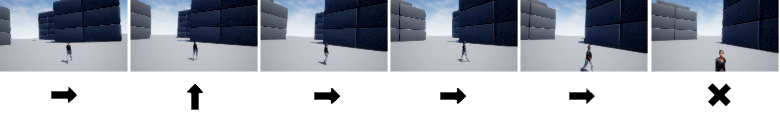
\includegraphics[width=\linewidth]{results/specific_situations/normalrun2-outofview.png}
    \caption{Stacked normal agent losing sight of the person}
    \label{im:normalrun2loses}
\end{figure}

Such situations explains the sudden drop 
in the reward distribution in Figure \ref{im:NormalDistro}, which happen because 
the agent deals with these states in later stages of an episode, as seen in Figure \ref{im:NormalPaths}.

A potential explanation could be the fact that a combination of an increased state-space 
by the stacking of images and the ability to perceive movements better when the drone is 
positioned sideways is impeding the learning process. Positioning itself to the side at 
some point during the training process could lead to higher rewards for the agent. 
Once this behavior has been reinforced through a large number of training cycles, it is 
increasingly hard for the agent to unlearn this behavior. This is especially the case considering 
that the DQN samples from a the larger replay buffer, reinforcing its memory that these 
actions lead to higher rewards. Furthermore, when these sequences of actions lead to 
later situations that are problematic, as seen in Figure \ref{im:normalrun2loses}, the 
increased state-space also impedes the agent even more to find better action sequences. 

Finally, looking at the single depth agent, the higher values in average return 
are being reflected in its behavior. 
The overall flight paths are smooth, even compared to the baseline. Its 
behavior is therefore very stable, further emphasizing its stability as was observed 
in its reward distribution (Figure \ref{im:NormalDistro}). Furthermore, no episode 
has ended in the agent losing sight of the person. 

In contrast to the other agents, the performance of the depth agent points to the simplifying
ability of using a depth map state-space. Additionally, the opposite can be said about the 
use of stacks of images. Increase in state-space in this manner is not helpful, at least in 
environments where they do not convey useful additional information
and the opposite effect with regards to the stacking the state-space. Comparing the agents 
to the baseline, indicates that there 
is a benefit of using RL methods combined with depth maps over the baseline in the task of 
follow-me behavior in an obstacle-free environment. Meanwhile, the use of normal images and 
stacked imaging do not provide useful additions to an agent in this context. 

\subsection{BlocksObstacles Environment}
In this section, a similar procedure
will be performed in the BlocksObstacles environment. Additionally, extra analysis 
regarding the behavior of the agents will be performed to get a grip on the bottlenecks of 
each specific agent. Furthermore, using 
the best working agent from the initial training and test runs, another agent will be 
trained using the same architecture, however with a different reward function. This will 
be performed in order to measure the impact of the reward function on the acquired 
behavior in the context of an environment that contains obstacles. The training 
procedure of all of these agents will be described, which will 
then be followed by the test results of each of them. 

\subsubsection{Training Process}
The training process has proceeded 
very similarly as in the BlocksNormal environment, with some extra points of attention. 
The exact process can be observed in 
Figure \ref{im:ObstaclesTraining}. The most 
notable point that can be seen is that the agents were not able to converge their 
average episode length to the maximum. Some performed better than others however, 
but none of them were able to exceed a 25 step average. An overall trend in all the 
metrics is a significant decrease in performance compared to the previous environment. 
This was to be expected looking at the drop in performance of the baseline in this newer
more complex environment. 

Another interesting point to note is that in the training average metric, we see that 
the stacked depth model was able to get to 
its convergent value the soonest. Especially the single normal image model underperformed 
compared to the other two models, which converged around a similar value. These features 
are also observed in the evaluation average return metrics, where the stacked depth 
image model reached the highest values the quickest. 

Finally, the maximum return of the agents did reach a convergence value of almost 50, 
meaning, again, that the agent's best episodes were the best that the agent could have 
done in these situations. At the same time, the minimum return of the evaluation 
episodes were much lower in comparison to the Blocks training cycle. These features 
show that the models have diverged much more to the extreme, especially in the lower ends, 
which resulted in the reduced performance. It is clear that the obstacles in the 
environment have had a worse effect on the minimum return and not so much on the 
highest return. \newline

\begin{Figure}
    \centering
    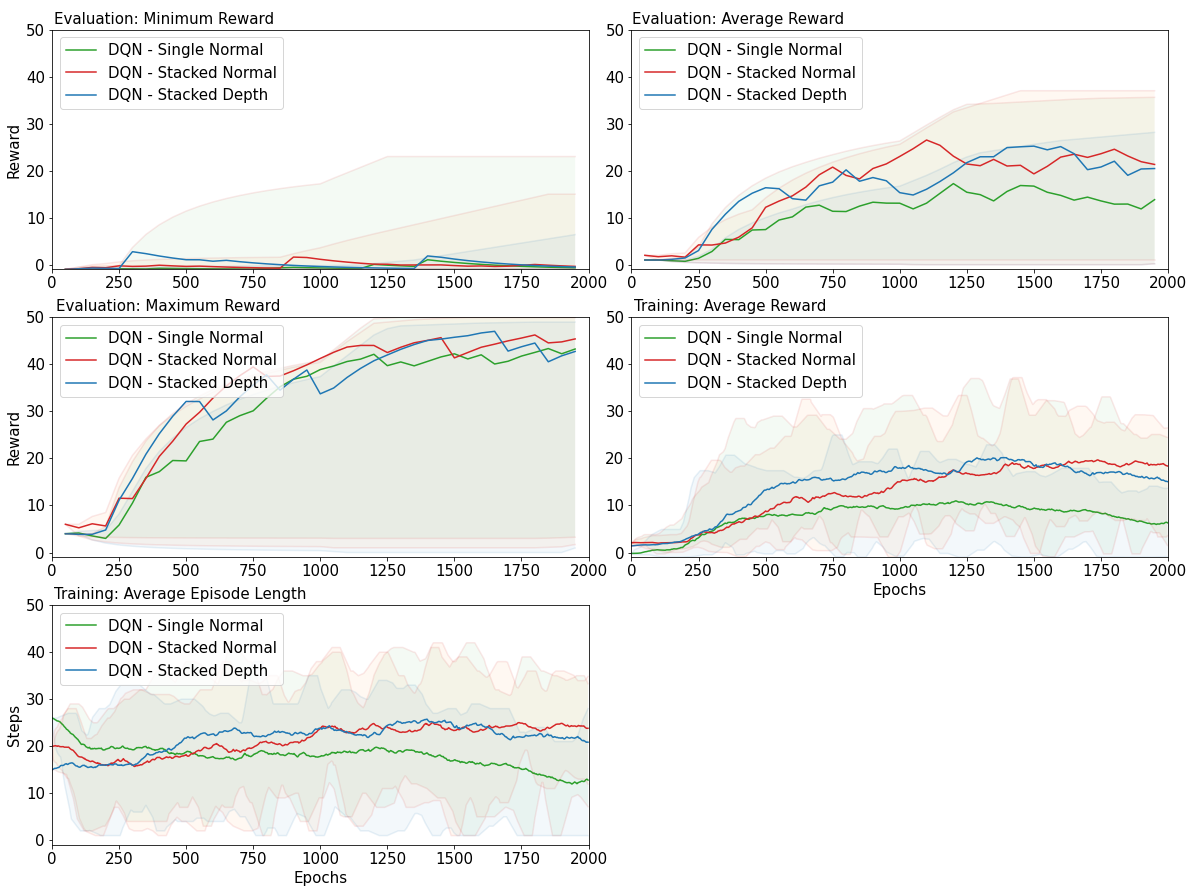
\includegraphics[width=\linewidth]{results/Training for BlocksObstacles.png}
    \captionof{figure}{Training Process in BlocksObstacles Environment}
    \label{im:ObstaclesTraining}
\end{Figure}

\subsubsection{Test Results}
Next, we will look at the results that were obtained from testing the models trained in 
BlocksObstacles environment in their own environment.
The test runs results for this can be seen in Table \ref{tab:ObstacleAVG}. This time, 
the expected return looking at the baseline degradation has also been included and the 
increase in performance compared to the expected return can also be seen. Finally, 
drop in performance compared to the last environment has also been added. 

\begin{table}[h]
    \centering
    \caption{Average return comparisons of test runs in BlocksObstacles}
    \label{tab:ObstacleAVG}
    \begin{tabular}{l|c|c|c|c}
    \multicolumn{1}{c|}{\textbf{Agent}} &
      \textbf{\begin{tabular}[c]{@{}c@{}}Average return\\(max. 50)\end{tabular}} &
      \textbf{\begin{tabular}[c]{@{}c@{}}Expected\\return*\end{tabular}} &
      \textbf{\begin{tabular}[c]{@{}c@{}}Difference\\ expected\\return**\end{tabular}} &
      \textbf{\begin{tabular}[c]{@{}c@{}}Difference\\ previous\\environment***\end{tabular}} \\ \hline
        Baseline             & 22.6 & n.a.   & n.a.  & -43.7 \% \\ \hline
        DQN - Single Normal  & 19.1 & 19.8 & -3.5 \% & -45.7 \%  \\
        DQN - Stacked Normal & 24.8 & 18.0 & \textbf{+37.7 \%} & \textbf{-22.3 \%} \\
        DQN - Stacked Depth   & \textbf{30.1} & 23.6 & +21.6 \% & -28.3 \%
    \end{tabular}
    \justify
    \small
    *The expected return has been calculated by using the degree 
    of degradation of the baseline going from the BlocksNormal to the 
    BlocksObstacles environment. In this case, it was 43.7\%.\newline
    **The percentage change in performance of the agents compared to the expected return. \newline
    ***The performance change for each agent compared to their counterpart in the 
    previous environment. 
\end{table}

These results show that the additions have had a positive influence on the 
performance of each consecutive agent implementation. Most notably, the use of stacked 
images has proven to be a more useful addition to the agent than previously, having 
the largest performance boost compared to the expected performance. Next to this, the 
fact that the performance difference of the stacked normal agent is significantly less than 
the single normal image also emphasizes this point. This is 
the case for both the comparison between the trained agent in the previous environment, 
but also for the comparison to the expected return. Meanwhile, the 
use of depth imaging had even better results. Although the difference has been slightly higher, 
the overall performance is still the highest. Seeing as the depth agents have been the best 
performing models in both environments, this slightly higher performance difference is not unsurprising. 
Overall, the stacked and depth agents outperformed the baseline performance, both 
in expected degradation and average return. 

These results show an initial clue that the use of 
RL algorithms can produce better performing models compared to the baselines. However, 
the state-representation used for these RL agents does matter. Further details will 
be elaborated upon in the next section. The specific behavioral elements that comprise these 
results will be analyzed next.  \newline

\noindent
\textbf{Reward Distribution} \newline
Looking at the rewards that each agent received on an average episode during 
the test run, which can be found in Figure \ref{im:ObstacleDistro}, we see some differences 
between the agent's behavior. 

\begin{Figure}
    \centering
    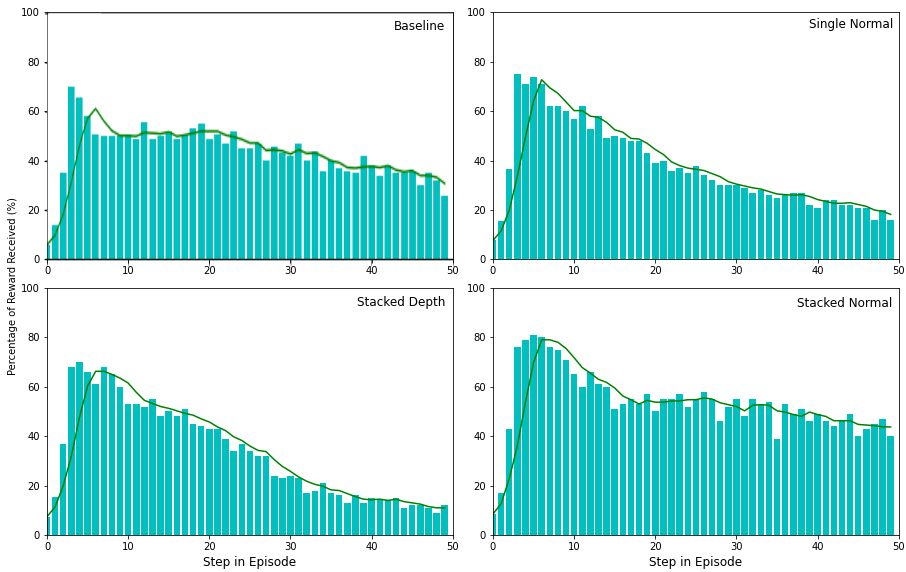
\includegraphics[width=\linewidth]{results/Reward Distribution of BlocksObstacles.png}
    \captionof{figure}{Reward distributions of models trained in BlocksObstacles environment}
    \label{im:ObstacleDistro}
\end{Figure}

The only difference that stacking the 
images does is a slightly larger reward during the intermediate steps of an 
episodes. This means that the agent is in goal states for a longer duration, before 
dropping to the lower values. However, both of these agents, in contrast to the stacked 
depth image model, have a downward trend. The longer the episode, the more 
the agent struggles with follow-me behavior, getting itself in crashes, losing 
sight of the person or simply being too far. However, the stacked depth image model can 
keep a steady value from the 15th frame onwards, despite a drop in the initial frames. 
It is clear that the previously observed stable behavior in the BlocksNormal environment 
is also appearing in this new environment. Again, the use of 
depth maps has been a beneficial aspect with regards to the agents developing overall 
stable behavior. Nonetheless, the 
depth agent still is struggling with later stages in an episode. The behaviors responsible 
for these distributions will be analyzed next.\newline

\noindent
\textbf{Behavior} \newline
The next analysis will look at the flight paths of the agents in the BlocksObstacles environment. 
The visualization for these paths can be seen in Figure 
\ref{im:ObstaclePathsDivided}. Additions to this figure are the areas in which the episode 
ends have taken place. These areas will be used to analyze the specific obstacles and 
situations the agents struggled with. The flight paths without these areas can be seen in 
Figure \ref{im:ObstaclePaths} in appendix \ref{appendixA}. \newline


\begin{SCfigure}[][h]
    \centering
    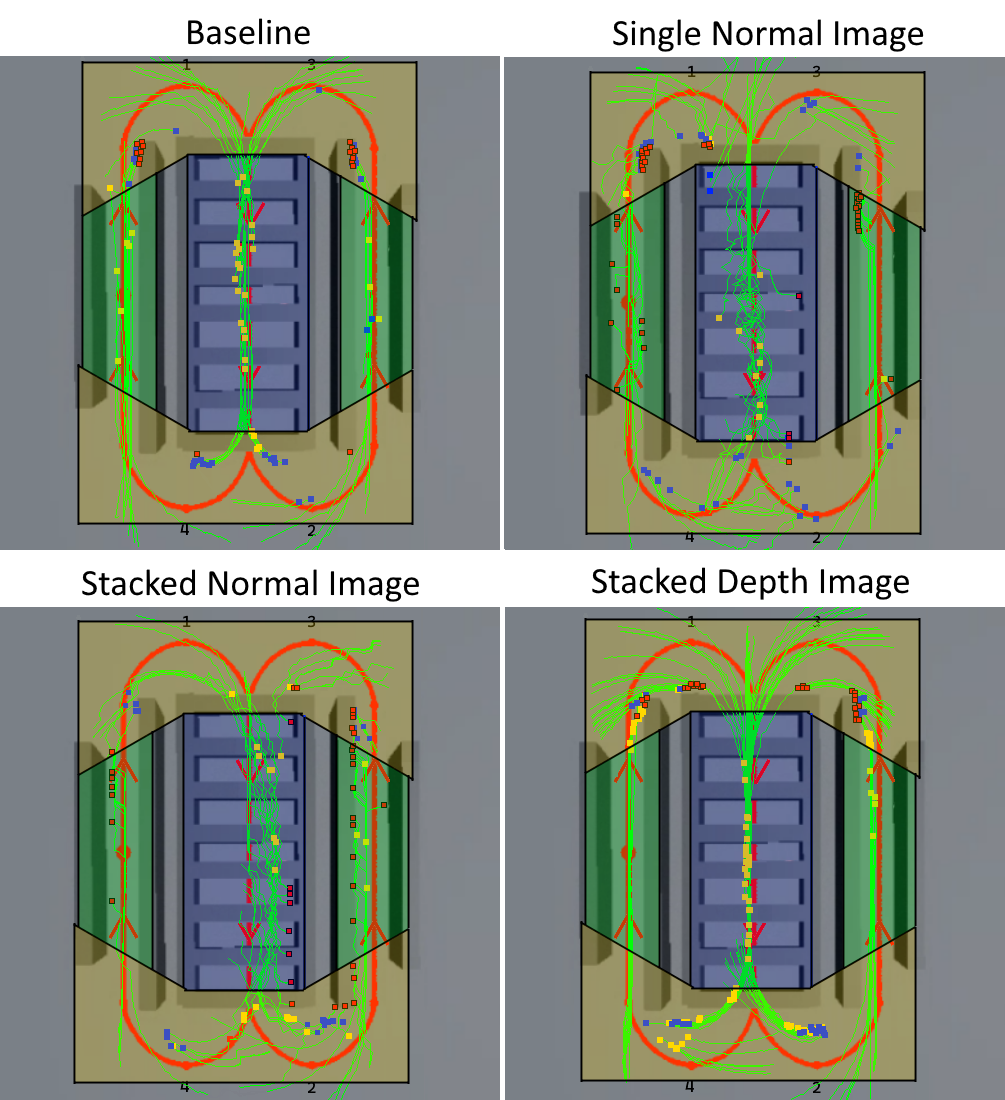
\includegraphics[width=0.66\linewidth]{results/summary-BlocksObstacles-PathsDivision.png}
    \captionof{figure}[Paths and episode ends of all the agents during a 100 episode test run in BlocksObstacles.]{Paths and episode ends of all the agents during a 100 episode test run in BlocksObstacles. 
    The green lines represent the flight paths of the agent.\newline\newline
    The areas correspond to the following situations: \newline
    Green = Tight hallways\newline
    Blue = Wide hallways \newline
    Yellow = Corners \newline\newline
    The dots correspond to the following episode ends: \newline
    Red = Collisions\newline
    Blue = Out of View \newline
    Yellow = Normal\newline\newline\newline\newline\newline\newline}
    \label{im:ObstaclePathsDivided}
\end{SCfigure}

From these images, the erratic behavior of the single normal image is visible again.
Furthermore, the stacked normal agent also repeats the pattern of behavior of 
positioning itself to the side of the person, however this time on the left side. 

Moving on to the next agent, the depth agent, the same pattern of smooth 
and stable flight paths can be observed as previously. Nonetheless, in this 
environment, the number of collisions and out of views has increased, as can 
be observed in Table \ref{tab:ObstacleEnds}. The specific behavior that resulted 
in these numbers will be further analyzed. This will be performed by looking at each 
type of obstacle separately. What ending location corresponded to what area
in this count can be observed in Figure \ref{im:ObstaclePathsDivided}. \newline

\begin{table}[h]
    \centering
    \caption{All of the unsuccesful ends inside of the BlocksObstacles environment test runs}
    \label{tab:ObstacleEnds}
    \begin{tabular}{l|c|c|c|c|c|c|c|c|c}
    \multicolumn{1}{c|}{\textbf{Agent}} &
      \multicolumn{3}{c|}{\textbf{Collisions}} &
      {\ul Total} &
      \multicolumn{3}{c|}{\textbf{Out of View}} &
      {\ul Total} &
      \textbf{\begin{tabular}[c]{@{}c@{}}Total\\ Overall\end{tabular}} \\ \hline
    \multicolumn{1}{c|}{\textit{Obstacle Type}} &
      \textit{Tight} &
      \textit{Wide} &
      \textit{Corners} &
      {\ul } &
      \textit{Tight} &
      \textit{Wide} &
      \textit{Corners} &
      {\ul } &
      \textbf{} \\ \hline
    Baseline       & 0  & 0 & 20 & {\ul 20} & 2 & 0 & 30 & {\ul 33} & \textbf{53} \\
    Single Normal  & 25 & 3 & 18 & {\ul 46} & 0 & 4 & 39 & {\ul 43} & \textbf{89} \\
    Stacked Normal & 17 & 7 & 14 & {\ul 38} & 0 & 0 & 24 & {\ul 24} & \textbf{62} \\
    Stacked Depth  & 0  & 0 & 25 & {\ul 25} & 0 & 0 & 24 & {\ul 24} & \textbf{49}
    \end{tabular}
\end{table}

\noindent
\textit{Hallways} \newline
The two types of hallways will be discussed further, starting with the wider hallway.
This type of situation has been comparatively the easier obstacle to deal with by 
the agents. Here, the only agents that have had problems have been the normal image 
agents. The fluctuant pattern of the single normal agent results in a sporadic end where 
it crashed against the wall. However, the other times the agent crashes or loses the person, 
it is as a 
run-up to the oncoming turn of the person. Looking at the flight patterns in 
Figure \ref{im:ObstaclePaths}, these mishaps are the results of the overall volatile 
behavior that this agent exhibits and not of a specific behavior pattern that was learned 
by the agent. 

Adding stacked images to this agent has shown the number of 
crashes in the wider hallway situation to be increased, while the times 
it lost sight of the person brought to zero. Looking at the flight 
patterns of this agent, much as in the previous environment, 
it clearly has a tendency to position itself to the side of the person. However, this time 
to the left. This, unfortunately, positions the drone in such a way that the walls are not 
visible anymore and a crash occurs. One such situation can be seen in Figure \ref{im:run2crashes}.

\begin{Figure}
    \centering
    \small
    Image: view of the drone $|$ Arrows: Action the agent performed
    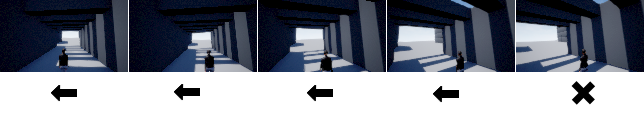
\includegraphics[width=\linewidth]{results/specific_situations/ObstaclesRun2-collision.png}
    \captionof{figure}{How the stacked normal agent crashes into the wall from behind}
    \label{im:run2crashes}
\end{Figure}

This behavior is a continuation of the problems during the learning process that was 
described in the previous section and is probably explained by a similar interpretation.
However, a possible explanation for why this time the preferred side of the agent to position 
itself differs, is a random choice early in the learning process. Developing this behavior 
early in the training process, an initial choice about which direction to go is made randomly.
It is then hard to unlearn this behavior, as mentioned earlier, because of the replay 
buffer sampling of the DQN. 

Looking at the tighter hallways, these situations have been a more difficult setting for some 
of the agents to 
deal with. Again, a similar division of the agents can be perceived, where the normal 
image agents have the most trouble with this situation, and the baseline and 
depth agent had no problems at all. For the two problematic agents, the pattern of 
behavior that leads to these failed endings are similar to those in the 
wider hallway. The increase in frequencies can be explained by the fact that 
the hallway is tighter, bringing about these situations sooner and more often. 
The baseline, which follows the path of the person very tightly, logically did not 
struggle with this situation. However, interesting to note is that this type of 
following is not achieved by the normal image agents, but has been by the depth 
agent, as reflected in the table. These findings additionally reinforce the 
hypothesis that the depth state-space allows for easier learning of behavior 
compared to the grayscale state-space. On top of that, the use of stacked state-
representation seems to ba a valuable addition in some contexts. Here, the 
environment and the type of pixel value matters.   \newline

\noindent
\textit{Corners} \newline
With regards to the corner situations, the variations to the agents proved to be 
useful additions that allowed them to better avoid the obstacles. 
However, the ability to perform significantly better than the baseline in this aspect is 
not observed. The single normal image had trouble completing 
any episode successfully, as can be seen in Table \ref{tab:ObstacleEnds}, 
struggling the most with corners, where a large portion of the collisions 
and out of view endings happened. This effect likely explained 
by the high volatility of its behavior that results in many different types of 
episode ends and beginnings. Overall, these results more strongly emphasize 
the problems of using single normal images as a state-representation, especially 
compared to the other agents. What's more, this agent does not show clear 
advantages over using the baseline method.  

The stacked agent was recorded having significantly less 
endings where the drone lost sight of the person. The number of times 
that a collision has occurred has decreased, but not by a large margin. This 
is explained by the fact that instead of having trouble in multiple places, the 
agent now is struggling at more specific moments, which in this case is the moment 
halfway through a turn. An example of the agent in this 
situation can be seen in Figure \ref{im:run2loses}. 

\begin{Figure}
    \centering
    \small
    Image: view of the drone $|$ Arrows: Action the agent performed
    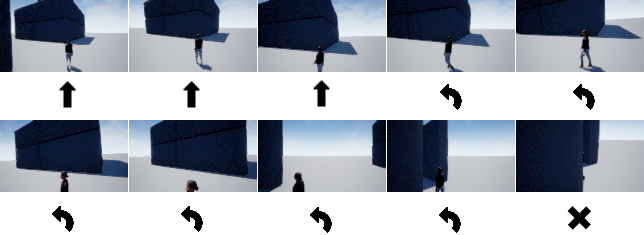
\includegraphics[width=\linewidth]{results/specific_situations/obstaclesrun2-outofview.png}
    \captionof{figure}{How the stacked normal agent loses the person}
    \label{im:run2loses}
\end{Figure}

It is apparent that the agent is upholding the behavior of following the person from the 
left. In some cases, it allows the drone to pass the first corner but holding on 
to this behavior leads to the problem of being blindsided 
by the wall that is appearing moments later. When in the situation of the last two 
frames of the figure, the agent is too close and unable to correct is behavior on time before 
losing sight of the person. In the clusters in the bottom left turns, the antithesis to this 
behavior is visible. Here the drone is too far away from the person to handle the final stages 
of the turns, resulting in losing the person. Finally, the top two turns have their own 
clusters, but in these situations, collisions are more apparent. This difference is 
because in the bottom turns, the drone is coming out of the 
wider hallway, which lends more space to position itself accordingly. In the top, 
the drone is coming out of the tighter hallway, lending less space for such manoeuvers. 
These results show that the stacking of images helps the agent in overall performance, meaning 
that the agent spends more time in goal states compared to the previous implementation. However, 
significant improvement in performance compared to the baseline is missing, and the increase in 
unsuccessful episode ends emphasize shortcomings in the learned behavior. 

Finally, the depth agent was struggling exclusively in the 
corners, mimicking the baselines behavior much more. As can be seen, in the top 
two corners, the agent has clusters of crashing, while in the lower two it is exclusively 
losing sight of the person. Again, this difference is explained by drone exiting either a 
wide or tight hallway. The baseline exhibits the same behavior. However, an interesting 
difference, is that the stacked depth agent has taught itself to position itself much 
closer to the person, as can be seen in Figure \ref{im:run3loses}. 

\begin{Figure}
    \centering
    \small
    Image: view of the drone $|$ Arrows: Action the agent performed
    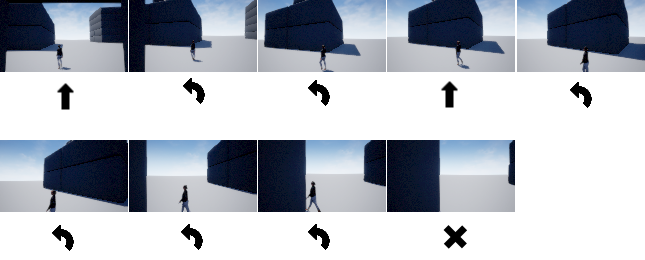
\includegraphics[width=\linewidth]{results/specific_situations/obstaclesrun3-outofview.png}
    \captionof{figure}{How the stacked depth agent loses the person}
    \label{im:run3loses}
\end{Figure}

It does so especially during the moments where the turn is occurring, in 
order to move past the first wall, so that it can focus on centering the person in its view. 
However, the issue is that after this has been done, the person is walking towards the 
second corner, which the drone is unable to see and correct for on time. 
What is interesting about this behavior is that it shows the ability of the agent to 
learn how to navigate itself around the first corner. It is struggling 
with the second stage of this process, because it is unable to observe the wall 
in order to act on time. These patterns are furthermore emphasized by the comparison of 
the flight paths seen in Figures \ref{im:ObstaclePathsDivided} and \ref{im:NormalPaths}.
For the general flight paths, Figure \ref{im:ObstaclePaths} in appendix \ref{appendixA} 
can be consulted. 

Interestingly, when looking at the flight paths of the depth agent in this environments 
compared to the BlocksNormal environments, it appears that the shape 
is different. The shape is clearly correcting for the obstacles 
in the former environments. It is unfortunately not always able to successfully finish 
this route, but the behavior does show that the agent is aware of the structures and 
has taught itself behavior to avoid it, albeit not completely infallible. 

A possible reason for why these situations are still so hard for the agent to deal with, 
could relate to shortcomings of the DQN agent. Considering the fact that DQNs 
are implemented using a memory buffer, they sample from their memory during the 
entire learning process. Seeing as most of the time, the person is walking 
straight, the largest proportion of experiences in the training batch will include 
transitions where the person is walking straight. Overall, this creates a bias 
in this replay buffer towards straight walking experiences, making it much harder 
for the agent to learn what to do with the turns. Nonetheless, compared to the 
baseline, these results have shown promising results for the capabilities of RL 
agents to learn behavior to avoid obstacles. \newline


\subsection{Warehouse Environment} \label{warehousetest}
The final environment in which tests have been performed, is the Warehouse environment. 
Here, the best performing agent from each environment is tested. Since these had 
different state-representation, the better working version of these agents in the Warehouse 
environment test runs will be retrained inside of this environment. 

\subsubsection{Training Process}
After the tests runs have been performed, for which the results and their corresponding 
elaboration can be seen in Section \ref{warehousetest}, the best performing model 
was the stacked depth model. The training process for this agent can be observed in 
Figure \ref{im:WarehouseTraining}.

\begin{Figure}
    \centering
    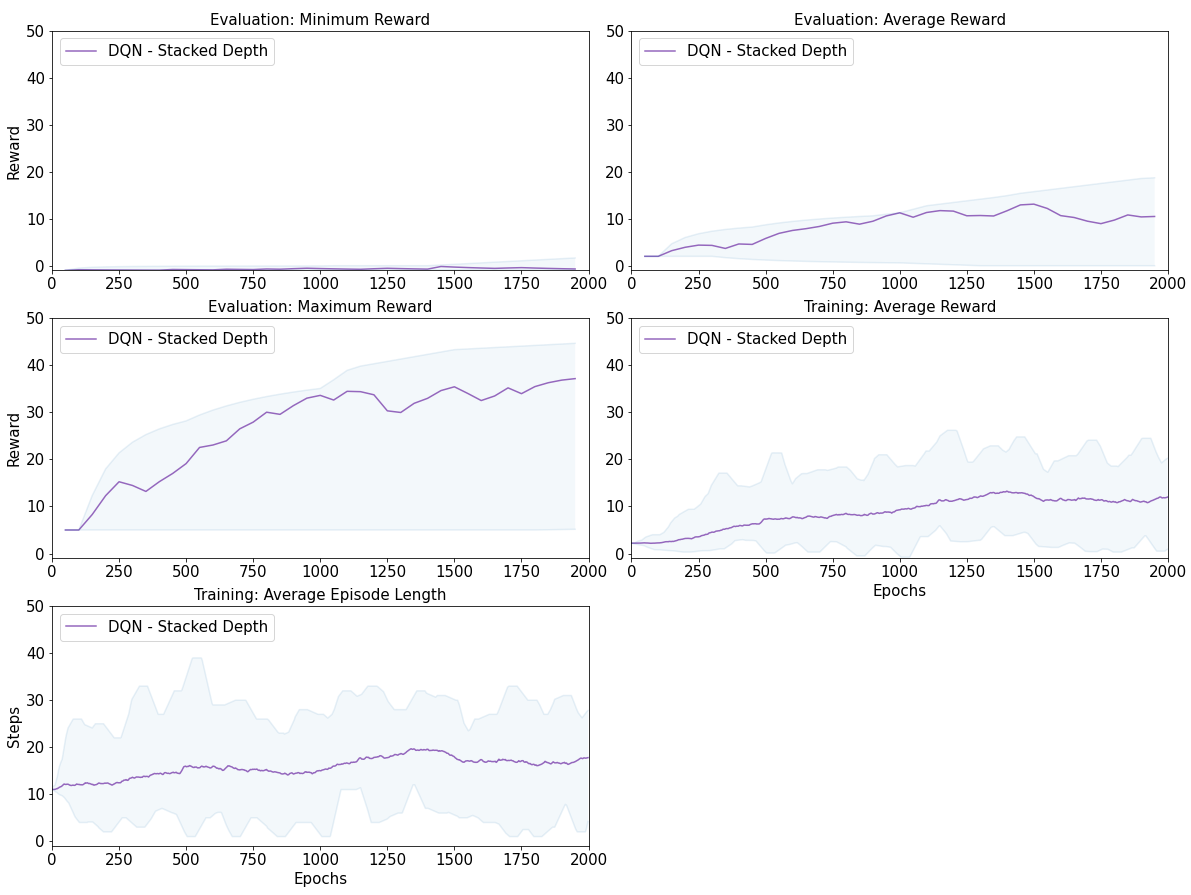
\includegraphics[width=\linewidth]{results/Training for Factory.png}
    \captionof{figure}{Training of Stacked Depth agent in Warehouse}
    \label{im:WarehouseTraining}
\end{Figure}

The results for the training of the stacked depth agent inside of the warehouse environment 
show a similar degradation in training performance as was perceived in the BlocksObstacles 
environment compared to the BlocksNormal. However, the degree of this degradation in this 
environment is lower. The average episode length during training time converged around a 
similar value than the BlocksObstacles environment, which was around 20 steps. 
Furthermore, both the average return during training time and evaluation time converged around 
a value of 10. These are only marginally lower than their counterparts in the BlocksObstacles 
environment, being 10 and 20 respectively. This is most likely cause by a lower minimum return, 
being almost never higher than zero. Next to this, the maximum return is also lowered, 
not reaching the maximum score of 50. 
The complexity of the environment has added increased difficulty for the learning process 
of the agent. The test results will elaborate on whether this also has an impact on the 
degree to which the agent behaves inside of the environment compared to other agents. 

\subsubsection{Test Results}
The final tests that have been performed all focus on the generalizability of 
RL agents to a new, more complex environment. This will be performed by using 
the degradation in performance that was observed in the baseline performing 
in the new environment. This drop in performance of the baseline is compared 
to the trained DQN - single depth agent in the BlocksNormal environment, the 
trained DQN - stacked depth agent in the BlocksObstacles, and a retrained DQN - 
stacked depth agent in the Warehouse environment. The average returns and the
compared performance drops can be observed \ref{tab:WareAVG}. 

\begin{table}[h]
    \centering
    \caption{Average return comparisons for the test runs in the Warehouse environment}
    \label{tab:WareAVG}
    \begin{tabular}{l|c|c|c|c}
    \multicolumn{1}{c|}{\textbf{Agent}} &
    \textbf{\begin{tabular}[c]{@{}c@{}}Average return\\(max. 50)\end{tabular}} &
    \textbf{\begin{tabular}[c]{@{}c@{}}Expected\\return*\end{tabular}} &
    \textbf{\begin{tabular}[c]{@{}c@{}}Difference\\ expected\\return**\end{tabular}} &
    \textbf{\begin{tabular}[c]{@{}c@{}}Difference\\ previous\\environment***\end{tabular}} \\ \hline

        Baseline                  & 9.9   & --  & -- & -56.2 \%       \\ \hline
        (Normal) Single Depth     & 11.5 & 11.5 &  0 \% & -72.7 \%     \\
        (Obstacles) Stacked Depth & 13.8 & 13.1 & +5.3 \% & -54.1 \%  \\
        (Warehouse) Stacked Depth & 21.6   & -- & +64.9 \% & -28.3 \%

    \end{tabular}
    \justify
    \small
    *The expected return has been calculated by using the degree 
    of degradation of the baseline going from the BlocksNormal to the 
    BlocksObstacles environment. In this case, it was 56.2\%.\newline
    **The percentage change in performance of the agents compared to the expected return. \newline
    ***The performance drop for each agent compared to their counterpart in the 
    previous environment. 
    \end{table}

Unsurprisingly, the baseline was the most underperforming agent of the set. However, 
the transferred agents, from both environments, only improved slightly. This is 
especially visible when compared to the expected return according to the degradation 
of the baseline. The single depth agent, trained in BlocksNormal, showed the exact 
amount of performance degradation as the baseline. Furthermore, the BlocksObstacles 
trained agent only improved slightly compared to the expected results. Nonetheless, 
the performance drop compared to their trained environments, can be seen to be the 
lowest for the BlocksObstacles trained agent. Nonetheless, the newly 
trained agent had the overall better performance. The added complexity of the 
obstacles formed a much larger problem for single depth agent. These results 
suggest that there has been little transfer of knowledge to the new domain. 
However, to further confirm these findings, a more in-depth look will be taken 
at their specific behavior. 


\begin{SCfigure}[][h]
    \centering
    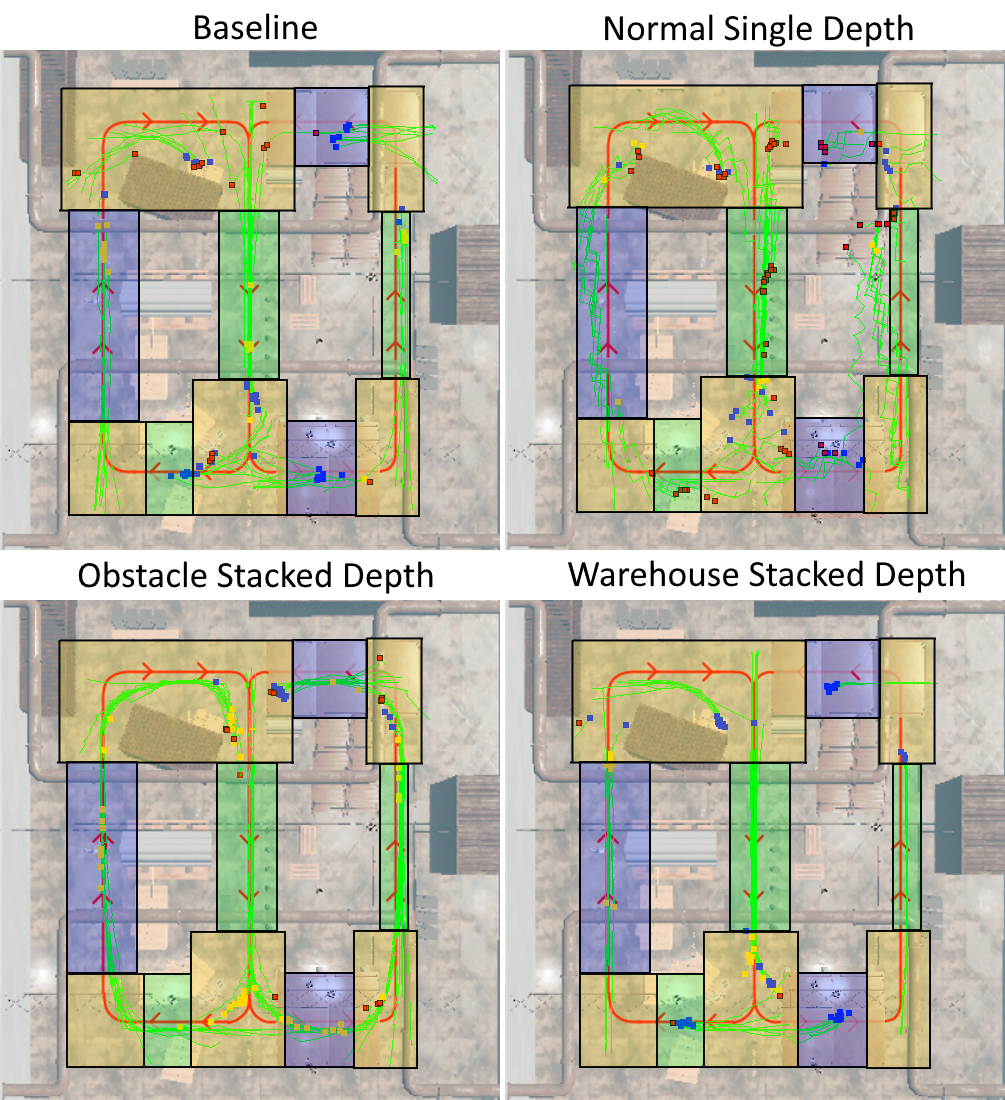
\includegraphics[width=0.66\linewidth]{results/WarehousePathsDivision.png}
    \captionof{figure}[Paths and episode ends of all the agents during a 100 episode test run in the Warehouse environment. ]{Paths and episode ends of all the agents during a 100 episode test run in the Warehouse environment. 
    The green lines represent the flight paths of the agent.\newline\newline\newline\newline\newline\newline\newline\newline
    The areas correspond to the following situations: \newline
    Green = Tight hallways\newline
    Blue = Wide hallways \newline
    Yellow = Corners \newline\newline
    The dots correspond to the following episode ends: \newline
    Red = Collisions\newline
    Blue = Out of View \newline
    Yellow = Normal}
    \label{im:FactoryPathsDivided}
\end{SCfigure}

Visible in Figure \ref{im:FactoryPathsDivided} is the fact that the depth images trained in environments with 
obstacles, showed the similar stable behavior that was observed in the previous 
two experiments, is visible in this one as well. However, what is interesting, is the 
fact that the agent trained in BlocksNormal was much more erratic. More surprisingly, 
is that a similar behavior that was observed in the stacked normal image agents, 
is now visible in this agent. The agent is trying to position itself to the left of 
the person throughout the episodes. This results in the increased crashes and 
out of views that is visible in Table \ref{tab:WareEnds}. This behavior 
only being expressed in this environment, is a sign that the agent is confused 
with the state-space. Not having been trained on any state that included obstacles, 
now clearly shows to be a problem for the agent in 
spaces where there are objects. This perturbs the agent so much as to illicit this unusual
behavior, with a bias towards the "move left" action. This shows that there is a limit to 
the generalizability 
capabilities of RL. Not having seen any instances of a given situation renders the agent 
incapable of acting accordingly. This explains the minimal 
transfer of its behavior to this new environment, as seen in Table \ref{tab:WareAVG}.
Further emphasizing this point, is Table \ref{tab:WareEnds}.

\begin{table}[h]
    \centering
    \caption{All of the unsuccesful ends inside of the Warehouse environment test runs}
    \label{tab:WareEnds}
    \begin{tabular}{l|c|c|c|c|c|c|c|c|c}
    \multicolumn{1}{c|}{\textbf{\begin{tabular}[c]{@{}c@{}}Agent\\(trained in:)\end{tabular}}} &
      \multicolumn{3}{c|}{\textbf{Collisions}} &
      {\ul Total} &
      \multicolumn{3}{c|}{\textbf{Out of View}} &
      {\ul Total} &
      \textbf{\begin{tabular}[c]{@{}c@{}}Total\\ Overall\end{tabular}} \\ \hline
    \multicolumn{1}{c|}{\textit{Obstacle Type}} &
      \textit{Tight} &
      \textit{Wide} &
      \textit{Corners} &
      {\ul } &
      \textit{Tight} &
      \textit{Wide} &
      \textit{Corners} &
      {\ul } &
      \textbf{} \\ \hline
    Baseline       & 0  & 1 & 15 & {\ul 16} & 5 & 13 & 42 & {\ul 60} & \textbf{76} \\
    BlocksNormal & 21 & 8 & 27 & {\ul 56} & 0 & 5 & 51 & {\ul 38} & \textbf{94} \\
    BlocksObstacles & 0 & 0 & 22 & {\ul 22} & 0 & 0 & 25 & {\ul 25} & \textbf{47} \\
    Warehouse & 1  & 0 & 2 & {\ul 3} & 11 & 12 & 45 & {\ul 68} & \textbf{71}
    \end{tabular}
\end{table}

What is interesting to see is that the two stacked depth agents performed better, but
their results are mixed. The stacked depth agent trained in the BlocksObstacles environment 
scored a lower average return, but had much less unsuccessful episode ends. These 
two results contradict each other. What seems to happen is that the retrained agent 
had much more trouble with not losing the person in the corners. Looking at the behavior, 
it is clearly visible that the agent is following the person much more closer than 
in the previous environment, as can be seen in Figure \ref{im:factorystackcomesclose}. 

\begin{Figure}
    \centering
    \small
    Image: view of the drone $|$ Arrows: Action the agent performed
    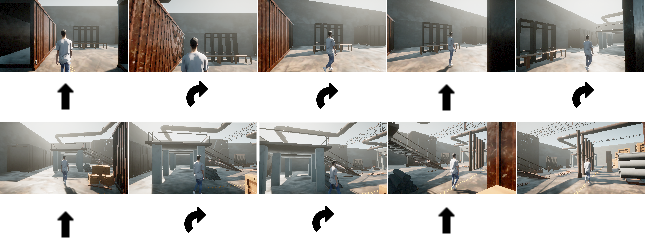
\includegraphics[width=0.9\linewidth]{results/specific_situations/obstaclerun3-comesclose.png}
    \captionof{figure}{How the stacked depth agent comes very close}
    \label{im:factorystackcomesclose}
\end{Figure}

This behavior is much more helpful with avoiding crashes and keeping the person in 
its FoV, however, it is not helpful for receiving reward, as is reflected in its 
average return. This is not reflected in the behavior of the stacked depth that 
has been retrained in the warehouse environment. However, this agent is impeded 
by the fact that it has not learned how to deal with these obstacles accordingly 
and keeps losing the person from its view. It has, however, taught itself to 
to avoid crashes, suggesting its ability to sense the obstacles and 
avoid them enough to not crash. Looking at the distribution of unsuccessful episode ends, 
both agents were 
mostly struggling in the situations of corners. The difference 
between the agents in the other two situations stems from the fact that the 
BlocksObstacles trained agent is closer to the person, leading to failed ends 
closer to the corners. On the other hand, the retrained agent is much farther 
and is therefore failing in similar situations nonetheless. 
These differences show that the best approach is 
still to train an agent in a specific environment. Doing this gives an agent 
the familiarity with the relevant situations to be able to behave accordingly. 
Nonetheless, transferring this knowledge from different environments still shows 
promising results, as the transferred agent behaved quite similarly as it had in 
the previous environment. Emphasizing this even further, is the fact that compared to the 
baseline, both agents performed significantly better. 

\subsection{Reward Functions Comparison}
In the final test, the reward function has been slightly adjusted as described in Section \ref{experiments}.
Using the best working agent from BlocksObstacles, which was the DQN - stacked depth agent, 
a new agent was trained using this new reward function. This reward function was a slight 
decrease in goal states. By making the margins of the goal distances to the 
person smaller, the reward function is made stricter. The overall reward function is thereby made even 
sparser. Testing this newly trained agent will give insights into the effect of the reward 
function on the acquired behavior. 

\subsubsection{Training Process}
The training process of this agent, as can be seen in Figure \ref{im:NewRewardTraining} in 
Appendix \ref{appendixA}, has proceeded almost identical to the training of the same agent 
using the normal reward function. These results are unexpected seeing as the reward function 
has been made even sparser. Seeing as there are even less states in which the agent receives 
a positive reward, it would be increasingly hard for the agent to find its way to these 
goal states. Considering this, the rewards should be overall lower, as the complexity of the 
problem has increased. Nonetheless, it appeared to converge at exactly the same values. These 
results potentially show that the agent learned the exact same behavior as before, leading 
to the similar learning results. This will analyzed below. 

\subsubsection{Test Results}
Having trained the agent using a new reward, a comparison can be made the 
same agent trained using the normal reward. This comparison can be seen in Table 
\ref{tab:RewardAVG}. 

\begin{table}[h]
    \centering
    \caption{Average return of the retrained agent with an adjusted reward function}
    \label{tab:RewardAVG}
    \begin{tabular}{l|c|c}
    \multicolumn{1}{c|}{\textbf{\begin{tabular}[c]{@{}c@{}}Reward \\ function\end{tabular}}} &
      \textbf{\begin{tabular}[c]{@{}c@{}}Average return\\ (max 50)\end{tabular}} &
      \textbf{Difference*} \\ \hline
    Normal Reward &
      39.1 &
      +65.7 \% \\
    Adjusted Reward &
      30.2 &
      --
    \end{tabular}
    \justify
    \small
    *The difference is calculated considering the expected reward for the Stacked Depth model as referenced 
    in Table \ref{tab:ObstacleAVG}. This expected reward was 23.6. 
\end{table}

This table shows that testing the agent using the adjusted reward has given a similar 
reward as the agent trained with a normal reward (Table \ref{tab:ObstacleAVG}). What is 
interesting, however, is that when testing this agent using the normal reward function, 
the average return is much higher. Seeing this increase by itself is not a surprising 
result, considering as the adjusted reward is much more strict compared to the normal 
one. These results show that the more precise a reward function is, the more focussed the 
agent becomes in keeping in these goal states. This is beneficial seeing as normally 
sparse reward functions make the learning process harder, decreasing reward. Important 
to note, is that there is a behavioral change, showing that although the training 
process was similar, the agents have learned different behaviors, which will 
be analyzed next. 

Looking more specifically at an average episode in Figure \ref{im:RewardDistro}, 
it is clear that this agent is better able to maintain the original level of 
rewards received in the early stages of the episode. 

\begin{Figure}
    \centering
    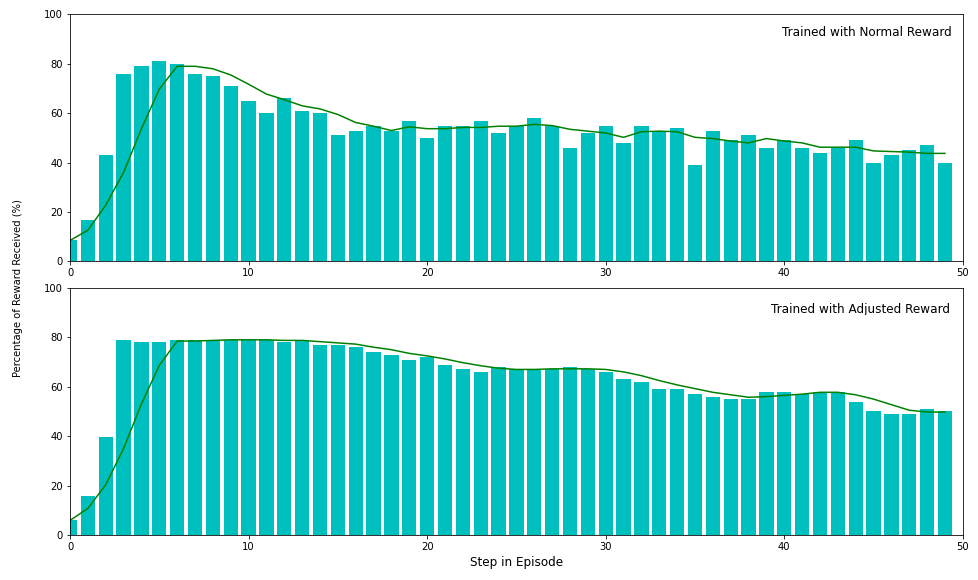
\includegraphics[width=0.8\linewidth]{results/Reward Distribution of NewRewards.png}
    \captionof{figure}{Reward Distribution of agent trained in BlocksObstacles with adjusted reward function.
    The collected rewards have been measured using the normal reward function.}
    \label{im:RewardDistro}
\end{Figure}

Next to this, the decreasing 
trend afterwards is less apparent than the agent trained using a normal reward. It is 
in these initial stages especially that this agent is earning more rewards compared to 
the normal agent. How this is achieved with behavior can be observed in Figure \ref{im:RewardPaths}. 

\begin{SCfigure}[][h]
    \centering
    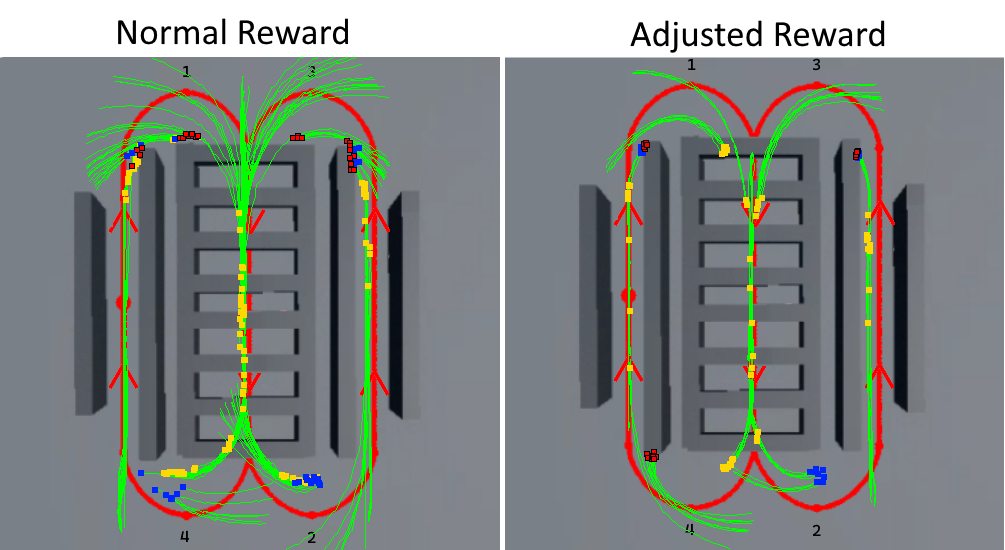
\includegraphics[width=0.66\linewidth]{results/BlocksObstacles Adjusted Rewards Paths.png}
    \captionof{figure}[Locations of each type of situation in the environments]{Locations of each type of situation in the environments\newline\newline\newline\newline
    The dots correspond to the following episode ends: \newline
    Red = Collisions\newline
    Blue = Out of View \newline
    Yellow = Normal}
    \label{im:RewardPaths}
\end{SCfigure}

As can be seen, the overall behavior seems similar. Many of the earlier mentioned behaviors
are apparent again, namely: keeping a stable flight path; staying close to the person's 
walking route; and having no trouble with the hallways situations. These aspects are further 
emphasized by the frequencies of unsuccessful episode ends as seen in Table \ref{tab:RewardEnds}.

\begin{table}[h]
    \centering
    \caption{Episode ends for the same agent trained using two different reward functions in BlocksObstacles}
    \label{tab:RewardEnds}
    \begin{tabular}{l|c|c|c}
    \textbf{Agent trained using:} & \textbf{Out of View} & \textbf{Collisions} & \multicolumn{1}{l}{\textbf{Total (/100)}} \\ \hline
    Normal Reward                 & 24                   & 25                  & 49                                        \\
    Adjusted Reward               & 21                   & 21                  & 42                                       
    \end{tabular}
\end{table}

However, a difference between the agents, is that the agent trained using 
the adjusted reward had overall less unsuccessful episode ends than before. However, 
what is more interesting, is the exact location in which these unsuccessful ends 
have happened. For the agent trained with the normal reward, there were multiple 
corners that were problematic. With collisions and out of view clusters at both 
the start and ending of the turn. However, this agent specifically had problems with 
the entrances and exits of the tight hallways. As can been seen in Figure \ref{im:RewardPaths}, 
the agent trained using the restrictive reward function mostly had collisions 
in the top two turns, in the first stages of exiting the tight hallway. An explanation 
for why it is struggling here is similar as in the BlocksObstacles environment. 
Leaving the tight hallways is hard as there is less room and the agent needs to 
explicitly move around it, which is a harder task in this situation than leaving the wider 
hallway. Next to this, entering the tight hallway is also a problem for the agent, seeing 
as there is another cluster of collisions in the bottom left turn. 

A positive point, nonetheless, is the fact that this agent is not struggling with the rest 
of the turn. This shows that the agent has learned to perform the rest of the turn successfully.
This is an improvement compared to the agent trained using the normal reward, as this agent 
had trouble with both corners in the top turns. Making sense of this, the agent has taught 
itself to follow the person much more tightly than the previous agents. Such behaviors 
are advantageous in situations where there is more room to make the turns. However, 
they also pose problems in the situations where there is no such room. It is apparent that 
the agent struggles more in these situations, and less in these others. This juxtaposition 
nonetheless shows an improvement in overall performance, and only a slight improvement in the
unsuccessful episode ends. Overall, however, this reward function has been a beneficial 
addition to the learned behavior of the agent. 

Concluding, changes to the reward function have a strong influence on the learned behavior. 
Considering the results of this experiment, minimal changes to the reward functions improved 
the behavior significantly. These findings further reinforce the aforementioned concepts that 
the reward signal is the foundation for the learned behavior of an RL agent. Other 
tests with the possibilities of different reward functions are still required, but are 
out of the scope of this thesis. 










        
        %todo: kerel wil iets over acties hebben


\section{Discussion}
In this section, we will discuss the overall conclusions that can be drawn from the 
results in perspective of the posed research questions (Section \ref{RQs}). 
After this, the limitations and problems of this thesis, 
together with possible future work that could be performed will be discussed. 

\subsection{Experiments and Research Questions}
Looking at the experiments, the previously posed research questions will be addressed. 
Each of these questions will be used as a perspective on the acquired results. 

\subsubsection{Directionality}
To start, the first research question investigated whether the use of stacked imaging 
improved the training process and performance in the Follow-Me task.
What has becomes clear, is that there is a benefit to stacking the frames. However, 
there is a caveat that needs to be added, which is that the context in which 
the agent is operating matters. 

Looking at the results, the stacked normal image 
agent outperformed the single image input model in the BlocksObstacles environment. 
However, in the BlocksNormal environment, it did not. The reason for this difference 
is that the stacking of the images as an input increased the state-space unnecessarily. 
When the images are stacked, the state-space is increased drastically. The 
expectation was that this increase would nonetheless provide sensible information that 
the drone could use to learn the required behavior faster and better. However, 
the lack of this observation in the obstacle-free environment, but the presence of it 
in the BlocksObstacles environment, confirms that this increase is only relevant 
in certain environments. Specifically, agents trained in environments that require 
the agent to handle obstacles are aided with this new state-representation. Such results 
emphasize that overall increases in state-spaces of an RL problem should be accompanied 
with valuable information for the agent to better optimize its reward. If this is already 
possible without this increased state-space, its learning process is only impeded. Such 
impediments lead to problematic behaviors, as observed in the results. In both 
environments that it was tested in, the agent taught itself a behavior that 
positions itself next to the person. In both environments, this lead to problems 
that the agent was not able to unlearn or deal with. This also lead to 
a high number of collisions or out of view moments, making this agent 
still prone to strong shortcomings. 

These results further reinforce the usefulness of using stacked imaging as an 
initial test for whether directionality in state-representation. Having been useful 
in initial deep RL domains \cite{rlsolvingatari}, its potential is further 
enforced in this thesis. At the same time, its shortcomings in more complex tasks 
are also laid bare. Seeing as this technique is a very straight-forward communication 
of the required information to the agent about moving objects, there are still questions 
about how to perform this more efficiently. This thesis has shown that such techniques 
are only beneficial when their impact on the state-space is mitigated by the possible 
benefits that they could add. In the specific task of follow-me behavior, this specific 
technique was not significantly more beneficial compared to its absence. However, these 
results nonetheless show promising results for the 
testing of more complex solutions in solving this task, such as the earlier presented 
RNN implementations \cite{RLenLSTMfordrone, LSTMinRL}. 

In conclusion, possible benefits from using state-representations that 
include information about the directionality of objects within the environment 
can provide valuable information to the agent to perform follow-me behavior. 
However, the overall benefits compared to using a single image are not convincing, 
and there is room for better techniques to be implemented to deal with this type of 
information. 

\subsubsection{Obstacle Avoidance} 
Next, the influence of depth maps in state-representation in the task of 
follow-me behavior has been tested. Overall, the results show 
implementing such information in the state-representation has significant 
benefits for the training process and its overall learned behavior. 

Looking at the results, the depth agents have either performed equally to, 
or even better than, the baseline in each of the environments. On top of this, 
the expected degradation in performance, was not matched by these agents, showing 
that they have been able to perform above what could be expected of them in 
each environment. Furthermore, compared to their normal image counterparts, the 
depth agents learned positive behavior the fastest compared to the others in some 
environments. These benefits stem from the fact that this change in state-space 
leads to simplifying the relevant information for the agent to behave well, the antithesis of 
the problems that stacking the images caused. 
To explain, two important aspects are required for the agent to perform follow-me behavior 
adequately. The drone should be able to sense the target object to follow and 
it should be able to sense its surroundings in order to see whether objects 
are in its way. The implementation of depth maps simplifies this latter 
information. Where normal images can represent walls in a variety of combinations 
of pixel values, depth maps represent these areas by their distances alone. 
With this, the information is simplified and it becomes easier for the 
drone to map such states to appropriate actions. 

These advantages translate to their learned behavior as well. In both the BlocksNormal
and the BlocksObstacles environments, this agent outperformed all the other agents. 
With very stable movements and 
keeping a close route to the person's walking path, this agent has been able to 
find better optima in its search for behavior that maximizes the reward. Compared to 
the normal image models, depth map agents had no problems with hallway situations, 
where no collisions have been recorded. On top of this, these agents also 
showed a slight improved ability to learn to avoid corners, having less problems 
with these situations than the other agents. Nonetheless, there are still points of 
improvements in this aspect, as these agents were not able to deal with corners 
adequately. 

The advantage to using depth maps over normal images has not been researched in 
the context of follow-me behavior. However, previous implementations using 
depth-maps to aid agents (including other vehicles) have been shown to be 
successful \cite{AirSimDroneNavigation, DepthAndStackResearch}. Their use  
has shown that agents can benefit from being able to sense surrounding objects 
when this is required for a task to be completed. In the context of follow-me 
behavior, this thesis has presented the benefits to this specific task. Nonetheless, 
there is still room to explore other technique that sense objects, as mentioned before \cite{acousticdronefollower,lidarinselfdrivingcar}.

Concluding, the results confirm the hypothesis that the addition of depth images 
as a means to replace a normal images, is a positive influence on the performance and 
training of a RL agent in the task of follow-me behavior. 

\subsubsection{Baseline}
Next, the third research question addressed the advantage of using RL methods 
over a heuristic inspired baseline. The results have shown that in cases where 
the perfect behavior has been adapted for, there are minimal differences between 
RL algorithms and agents that behave according to static rules. However, when 
adaptive behavior is required in exceptional situations, this difference is increased 
in the favor of RL method. 

Emphasizing this more strongly, the results have shown that in the BlocksNormal environment, 
where no obstacles are present, the set of rules that determine the baseline's behavior 
are sufficient to behave adequately. RL agents, in this context, are nonetheless able to 
match this. However, when obstacles have been added, this changes. Baseline methods 
are unable to adapt, as expected, and the advantages of trained RL agents are visible. 
Their degradation in performance was much less compared to the baselines degradation, showing 
that these agents have been able to adapt their behavior accordingly in these new situations. 
This is further explained by the behaviors that the agents exhibited. 
The baseline agent, with its static behavior, has specific problems that it is 
not able to deal with. However, RL agents have shown an ability to adapt 
their behavior to different situations, resulting in better performances overall. 
Even though problems persisted with the RL agents, their ability to adapt 
according to their environment shows the clear advantage that RL has over 
heuristic based approaches where new programming is required for each new 
situation. 

Looking at previous research in object tracking using similar heuristic rules \cite{DroneFollowUsingPhone, acousticdronefollower, DroneFollowMobileObject, VisualGPS},
it becomes clear that adaptive behavior is still very relevant, especially for 
dynamic object tracking tasks. Even though additional technologies improve 
the conditions in which these agents operate, their static foundation still 
can be improved using adaptive learning methods, such as RL. This thesis has 
presented the clear benefits of training such agents in these settings as opposed 
to adapting baselines. 

In conclusions, these findings reinforce the 
hypothesis that RL do provide advantages over more pre-programmed approaches in 
performing follow-me behavior. 

\subsubsection{Generalizability}
Finally, the last research question studied the generalizability of RL from simpler 
environments to more complex environments. Agents trained in simpler environments, have been 
tested in a more complex environment to see how much of the behavior has been transferred 
to these new situations. The results showed that RL methods do 
have generalizability, but show limits to the situations it can correctly infer. 

Specifically looking at the agent that was trained in BlocksNormal, it showed that 
it was strongly perturbed in the Warehouse environment. Not having 
seen these states during training, the agent is unfamiliar with these new states 
and performs unexpected behavior that was not 
observed in the training environment. RL agents trained in obstacle-free environments 
are therefore unable to generalize their behavior to environments where obstacles 
are present. On the other hand, the agent trained in BlocksObstacles, showed much 
more behavior transfer to the Warehouse environment. Although its
average return showed marginal improvement, its behavior showed many similarities 
when compared to its performance in its own environment. The difference between 
training an agent and transferring its knowledge seemed marginal as well, giving 
promising results for the ability of RL to generalize learned behavior to more 
complex situations. 

Looking at earlier attempts at transferring behavior to new environments \cite{DroneRLUsingTransferLearning}, 
shortcomings were observed regarding state-space. The use of normal images 
showed reduced generalizability to new environments, especially when colors and 
textures were changed. In this study, the agents have been trained using depth imaging 
and their generalizability has been tested. The generalizability of these agents has 
shown promising results and show the ability of RL agents to perform adaptive 
behavior to more complex environments. Furthermore, tests about whether RL agents 
are able to be trained in simple environments, and transfer this behavior to more 
complex environments have been missing. 

Many studies have shown problems with 
models developed in simulation environments being transferred to the real world \cite{DroneRLUsingTransferLearning, RLenLSTMfordrone}. 
The increase in complexity in this transition is an impediment to many agents that 
have been developed for a variety of tasks. The development of adaptive agents that 
are able to flexibly transfer behavior to real-world application is still relevant. 
The findings of this study have shown potential indications that RL agents are 
able to perform such adaptable behaviors. 

The findings in this study further emphasize the 
utility of using RL agents in developing more general behavior to be used in 
a variety of situations. Especially considering the comparison with baselines, 
where such behavior require pre-programming. 


\subsection{Limitations and Future Work}
Some topics of improvement require further attention. This dissertation has 
shown the overall usefulness of RL in the task of follow-me behavior. However, 
some elements could use some more in-depth research. 

To start, even though the implementation of the DQN has shown promising results 
in learning behavior, there might be some drawbacks to using this type of learning. 
As has been seen in the results, the best performing agents still struggled with 
some situations. The reasons for these struggles are most likely caused by a bias in 
the memory buffer of the DQN agent towards situations that occur most often. 
This lends itself to studying whether training methods that include weight experiences, 
such as Prioritized Experience Replay \cite{prioritizedreplay}, could improve 
the behavior sufficiently to solve these issues. Furthermore, other agents learn 
using different methods, some of which being without a memory buffer \cite{A3C, PPO,SAC}. 
Potential future work could investigate whether these agents are valuable additions 
in improving the drone's behavior. 

Furthermore, the action space of the agent in this study has been turned discrete 
as a means to implement the DQN. Relevant actions have been included in order to 
perform basic movements in the environment. However, there is also the possibility 
to give agents full control of the continuous actions space of a drone. Specific 
directions and velocities could be variables that an agent could take control of 
to ensure more stable behavior. Additional, vertical flight paths as a means to improve 
person centering could also be implemented. The ability of RL agent to take control of 
continuous action spaces has been shown previously \cite{FrontalViewRL, AirSimDroneNavigation}. 
Interesting research could be performed about whether RL agents with abilities to 
handle continuous spaces \cite{A3C, PPO, SAC, DDPG} could perform follow-me behavior. 

Moving on, as shown in the results, the reward function is a fundamental element 
when it comes to the behavior that is learned. For RL algorithms, the goal behavior is 
synonymous with maximizing the reward function \cite{RLBook}, meaning that the reward 
function has an essential relationship with the learned behavior. In this thesis, 
the choice has been made for a sparse reward function because of the possible problems 
that could be encountered with using the alternative manually shaped reward functions 
\cite{sparserewardsarebetter,nonsparserewardissuboptimal}. However, as shown in the 
results, even within the specific reward function created in these experiments, there 
is room for further shaping. Restricting the rewards even more changed the behavior 
of the agent measurably. There could still be different reward functions that could 
improve overall behavior in ways as to reduce collisions and other problems. Such 
investigation have fallen outside of the scope of this research, but they could 
be an inspiration for future work in developing follow-me behavior. 

Next, the techniques used to test different state-representations have shown 
promising results, but more research could be done in different types of 
techniques. As mentioned before, the use of stack imaging is a straight-forward 
approach to providing an agent with information about dynamic objects \cite{rlsolvingatari,DepthAndStackResearch}, 
however, there are still others that could improve overall results. Different 
architectures of RNNs could be implemented to improve these skills. Furthermore,
with the goal of further deployment in real world applications, there is still 
considerable room for future work into different methods of creating depth maps, 
as there is always some margin of error in such methods \cite{lidarinselfdrivingcar, stereovision, DepthFromMonocularImage}.

Finally, one shortcoming of RL algorithms is that they suffer from results that 
are hard to reproduce \cite{RLisSuperannoying}. 
RL is extremely sensitive to changes in the hyperparameters leading to completely 
different results. Considering the fact that in the scope of this thesis, no 
hyperparameters search has been performed, it is not clear that these results 
are completely optimal. However, since the goal has been to test the agents 
in comparison to baseline methods, these problems fall out of the scope of this thesis, 
but could potentially pose problems in further deployment of similar models. 

\subsection{Conclusion}
To conclude, this thesis has investigated to what extent the use of Reinforcement Learning
is a viable method for follow-me behavior using an autonomous drone. The 
results have shown that there is potential in using RL methods for this task, especially 
over straight-forward static approaches. Furthermore, implementing state-representations 
that incorporate information about the dynamic movements of objects and their distances, 
show strong advantages over RL algorithms that solely rely on camera inputs. Adding to 
this, the abilities of RL agents to transfer their behavior to more complex environments, show 
potential for the development of agents that teach themselves more general behavior to be 
applied in a larger variety of situations. Even though 
future work is required before deployment into real-world applications is possible, 
the use of RL shows strong advantages in the adaptive decision-making processes and generalizability. 

        \newpage
    }
    \bibliographystyle{ieeetr}
    \bibliography{Contents/references.bib}

    \appendix
\section{Appendix A} \label{appendixA}


\begin{Figure}
    \centering
    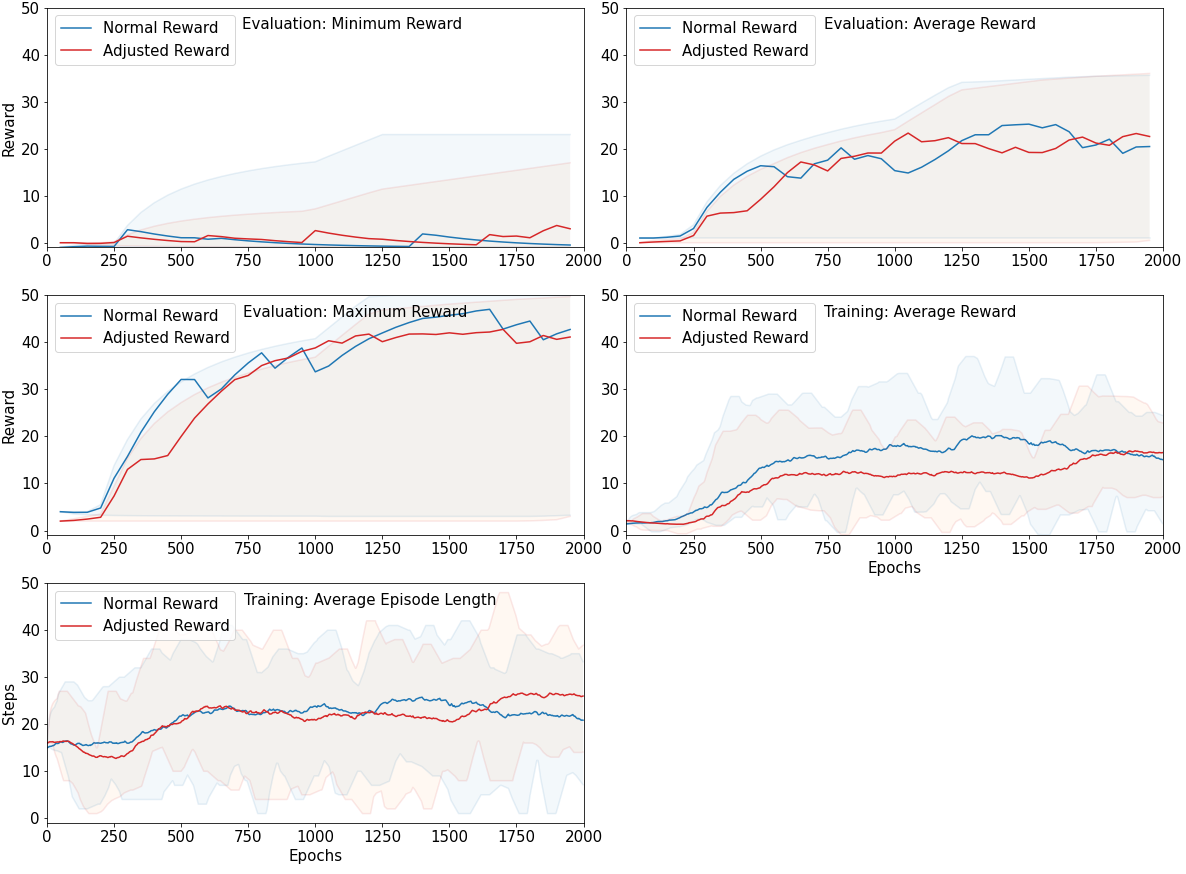
\includegraphics[width=\linewidth]{results/NewReward Training in BlocksObstacles.png}
    \captionof{figure}{Training Process in BlocksObstacles Environment with Adjusted Reward}
    \label{im:NewRewardTraining}
\end{Figure}


\begin{SCfigure}
    \centering
    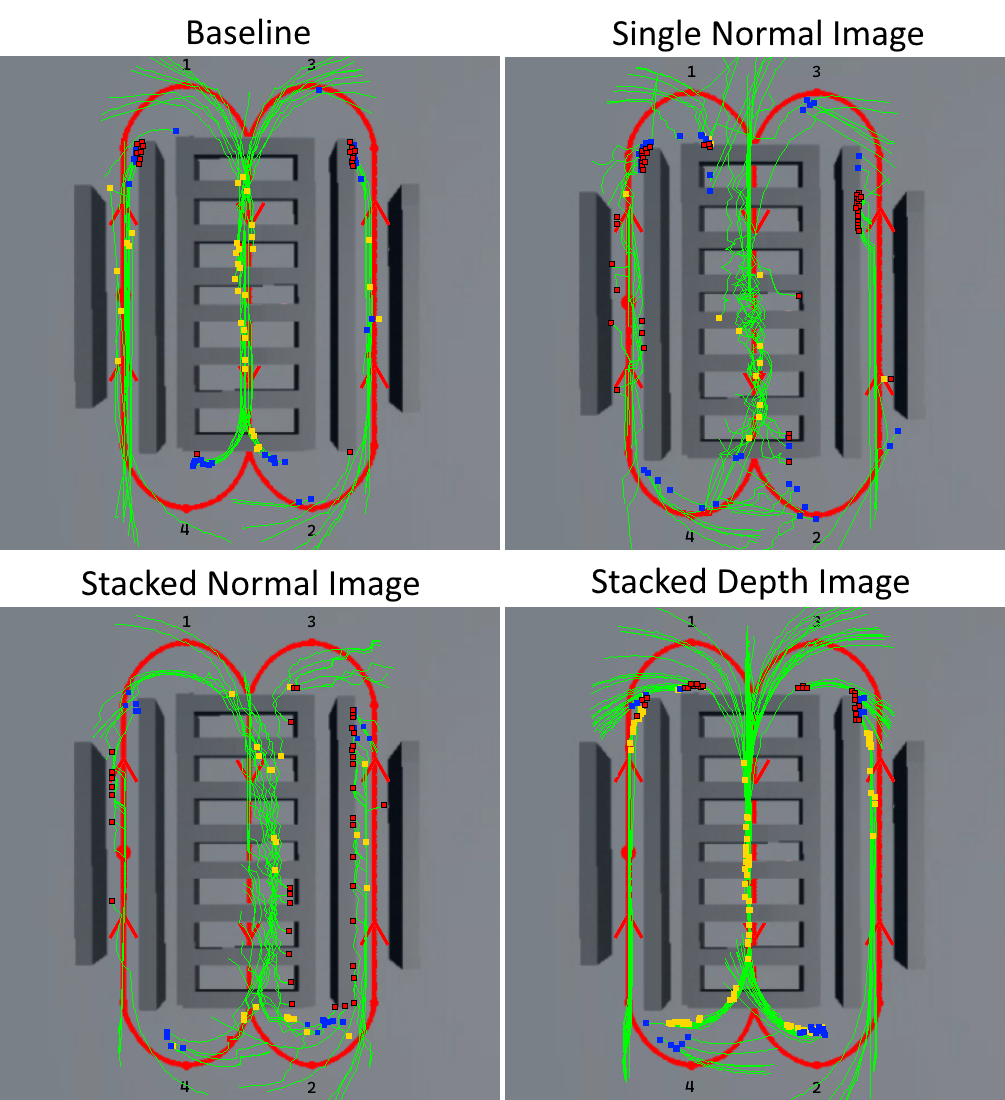
\includegraphics[width=0.66\linewidth]{results/summary-BlocksObstacles-PathsNew.png}
    \captionof{figure}[Overview of paths in BlocksObstacles environment]{Overview of paths in BlocksObstacles environment\newline\newline\newline\newline\newline\newline\newline\newline\newline\newline\newline\newline\newline\newline\newline\newline\newline
    The dots correspond to the following episode ends: \newline
    Red = Collisions\newline
    Blue = Out of View \newline
    Yellow = Corners}
    \label{im:ObstaclePaths}
\end{SCfigure}



\begin{SCfigure}
    \centering
    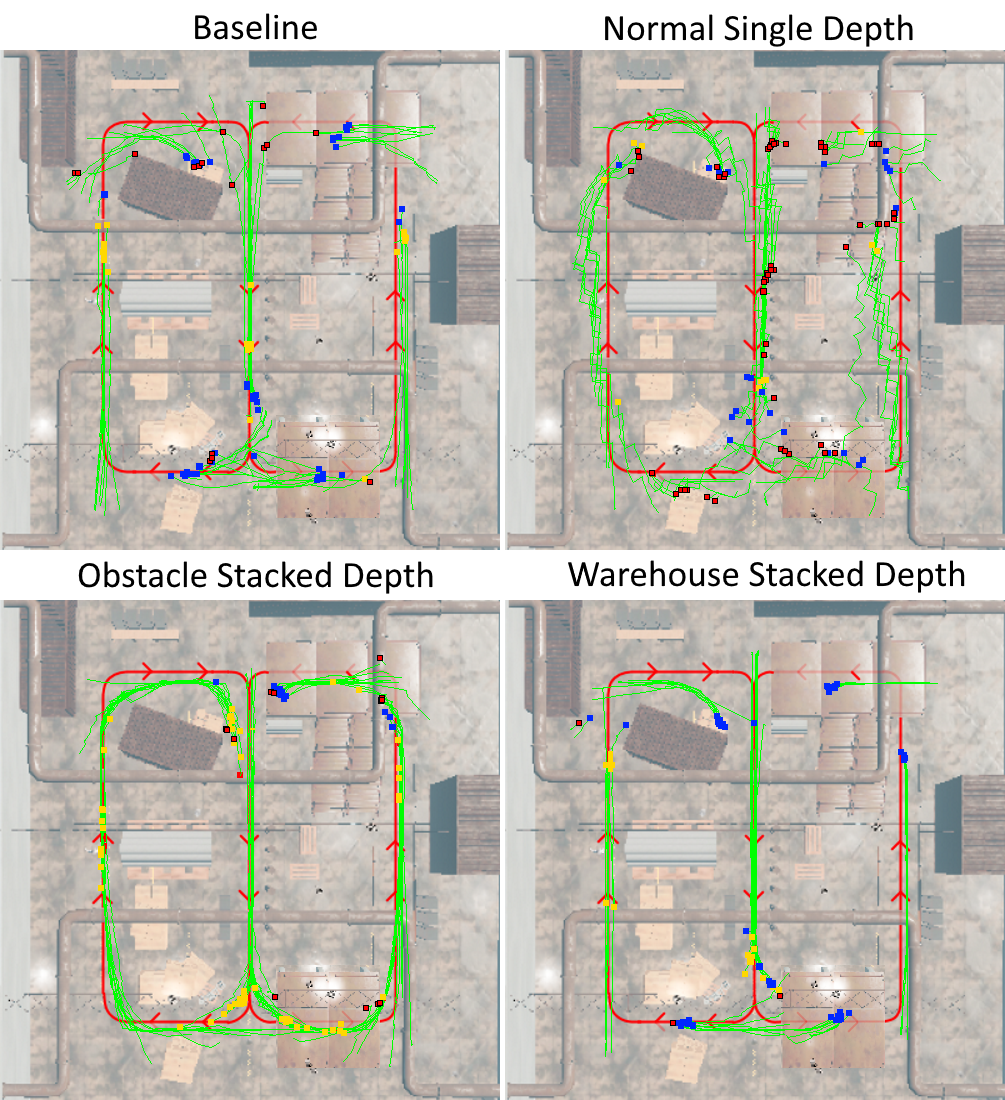
\includegraphics[width=0.66\linewidth]{results/WarehousePaths.png}
    \captionof{figure}[Overview of paths in Warehouse environment]{Overview of paths in Warehouse environment\newline\newline\newline\newline\newline\newline\newline\newline\newline\newline\newline\newline\newline\newline\newline\newline\newline\newline
    The dots correspond to the following episode ends: \newline
    Red = Collisions\newline
    Blue = Out of View \newline
    Yellow = Corners}
    \label{im:FactoryPaths}
\end{SCfigure}




    \section{Acknowledgements}
    \setstretch{1.5}
    I would like to thank dr. ir. R. Poppe for his help and feedback throughout the 
    research process. I would also like to thank ML6, and specifically Laurens Weijs, 
    for the opportunity to perform such an interesting research project and the 
    continued guidance throughout the whole process. Furthermore, I would like to 
    thank Raphael Fortunato for the companionship during the last nine months throughout the 
    whole project and for showing me the strong benefits of using open-source software
    and linux based systems. 
    I would also like to thank Sofie Bracher for her help with making a very specific
    figure. Finally, I would like to thank Tine Meerdink, whose strong academic and 
    writing skills have helped me think critically about my thesis and for the general 
    support during the last months. 



\end{document}  
